\PassOptionsToPackage{unicode=true}{hyperref} % options for packages loaded elsewhere
\PassOptionsToPackage{hyphens}{url}
%
\documentclass[
  ignorenonframetext,
]{beamer}
\usepackage{pgfpages}
\setbeamertemplate{caption}[numbered]
\setbeamertemplate{caption label separator}{: }
\setbeamercolor{caption name}{fg=normal text.fg}
\beamertemplatenavigationsymbolsempty
% Prevent slide breaks in the middle of a paragraph:
\widowpenalties 1 10000
\raggedbottom
\setbeamertemplate{part page}{
  \centering
  \begin{beamercolorbox}[sep=16pt,center]{part title}
    \usebeamerfont{part title}\insertpart\par
  \end{beamercolorbox}
}
\setbeamertemplate{section page}{
  \centering
  \begin{beamercolorbox}[sep=12pt,center]{part title}
    \usebeamerfont{section title}\insertsection\par
  \end{beamercolorbox}
}
\setbeamertemplate{subsection page}{
  \centering
  \begin{beamercolorbox}[sep=8pt,center]{part title}
    \usebeamerfont{subsection title}\insertsubsection\par
  \end{beamercolorbox}
}
\AtBeginPart{
  \frame{\partpage}
}
\AtBeginSection{
  \ifbibliography
  \else
    \frame{\sectionpage}
  \fi
}
\AtBeginSubsection{
  \frame{\subsectionpage}
}
\usepackage{lmodern}
\usepackage{amssymb,amsmath}
\usepackage{ifxetex,ifluatex}
\ifnum 0\ifxetex 1\fi\ifluatex 1\fi=0 % if pdftex
  \usepackage[T1]{fontenc}
  \usepackage[utf8]{inputenc}
  \usepackage{textcomp} % provides euro and other symbols
\else % if luatex or xelatex
  \usepackage{unicode-math}
  \defaultfontfeatures{Scale=MatchLowercase}
  \defaultfontfeatures[\rmfamily]{Ligatures=TeX,Scale=1}
\fi
% use upquote if available, for straight quotes in verbatim environments
\IfFileExists{upquote.sty}{\usepackage{upquote}}{}
\IfFileExists{microtype.sty}{% use microtype if available
  \usepackage[]{microtype}
  \UseMicrotypeSet[protrusion]{basicmath} % disable protrusion for tt fonts
}{}
\makeatletter
\@ifundefined{KOMAClassName}{% if non-KOMA class
  \IfFileExists{parskip.sty}{%
    \usepackage{parskip}
  }{% else
    \setlength{\parindent}{0pt}
    \setlength{\parskip}{6pt plus 2pt minus 1pt}}
}{% if KOMA class
  \KOMAoptions{parskip=half}}
\makeatother
\usepackage{xcolor}
\IfFileExists{xurl.sty}{\usepackage{xurl}}{} % add URL line breaks if available
\IfFileExists{bookmark.sty}{\usepackage{bookmark}}{\usepackage{hyperref}}
\hypersetup{
  pdftitle={Simple \& Multiple Correspondence Analyses},
  pdfauthor={Derek Beaton},
  pdfborder={0 0 0},
  breaklinks=true}
\urlstyle{same}  % don't use monospace font for urls
\newif\ifbibliography
\usepackage{color}
\usepackage{fancyvrb}
\newcommand{\VerbBar}{|}
\newcommand{\VERB}{\Verb[commandchars=\\\{\}]}
\DefineVerbatimEnvironment{Highlighting}{Verbatim}{commandchars=\\\{\}}
% Add ',fontsize=\small' for more characters per line
\usepackage{framed}
\definecolor{shadecolor}{RGB}{248,248,248}
\newenvironment{Shaded}{\begin{snugshade}}{\end{snugshade}}
\newcommand{\AlertTok}[1]{\textcolor[rgb]{0.94,0.16,0.16}{#1}}
\newcommand{\AnnotationTok}[1]{\textcolor[rgb]{0.56,0.35,0.01}{\textbf{\textit{#1}}}}
\newcommand{\AttributeTok}[1]{\textcolor[rgb]{0.77,0.63,0.00}{#1}}
\newcommand{\BaseNTok}[1]{\textcolor[rgb]{0.00,0.00,0.81}{#1}}
\newcommand{\BuiltInTok}[1]{#1}
\newcommand{\CharTok}[1]{\textcolor[rgb]{0.31,0.60,0.02}{#1}}
\newcommand{\CommentTok}[1]{\textcolor[rgb]{0.56,0.35,0.01}{\textit{#1}}}
\newcommand{\CommentVarTok}[1]{\textcolor[rgb]{0.56,0.35,0.01}{\textbf{\textit{#1}}}}
\newcommand{\ConstantTok}[1]{\textcolor[rgb]{0.00,0.00,0.00}{#1}}
\newcommand{\ControlFlowTok}[1]{\textcolor[rgb]{0.13,0.29,0.53}{\textbf{#1}}}
\newcommand{\DataTypeTok}[1]{\textcolor[rgb]{0.13,0.29,0.53}{#1}}
\newcommand{\DecValTok}[1]{\textcolor[rgb]{0.00,0.00,0.81}{#1}}
\newcommand{\DocumentationTok}[1]{\textcolor[rgb]{0.56,0.35,0.01}{\textbf{\textit{#1}}}}
\newcommand{\ErrorTok}[1]{\textcolor[rgb]{0.64,0.00,0.00}{\textbf{#1}}}
\newcommand{\ExtensionTok}[1]{#1}
\newcommand{\FloatTok}[1]{\textcolor[rgb]{0.00,0.00,0.81}{#1}}
\newcommand{\FunctionTok}[1]{\textcolor[rgb]{0.00,0.00,0.00}{#1}}
\newcommand{\ImportTok}[1]{#1}
\newcommand{\InformationTok}[1]{\textcolor[rgb]{0.56,0.35,0.01}{\textbf{\textit{#1}}}}
\newcommand{\KeywordTok}[1]{\textcolor[rgb]{0.13,0.29,0.53}{\textbf{#1}}}
\newcommand{\NormalTok}[1]{#1}
\newcommand{\OperatorTok}[1]{\textcolor[rgb]{0.81,0.36,0.00}{\textbf{#1}}}
\newcommand{\OtherTok}[1]{\textcolor[rgb]{0.56,0.35,0.01}{#1}}
\newcommand{\PreprocessorTok}[1]{\textcolor[rgb]{0.56,0.35,0.01}{\textit{#1}}}
\newcommand{\RegionMarkerTok}[1]{#1}
\newcommand{\SpecialCharTok}[1]{\textcolor[rgb]{0.00,0.00,0.00}{#1}}
\newcommand{\SpecialStringTok}[1]{\textcolor[rgb]{0.31,0.60,0.02}{#1}}
\newcommand{\StringTok}[1]{\textcolor[rgb]{0.31,0.60,0.02}{#1}}
\newcommand{\VariableTok}[1]{\textcolor[rgb]{0.00,0.00,0.00}{#1}}
\newcommand{\VerbatimStringTok}[1]{\textcolor[rgb]{0.31,0.60,0.02}{#1}}
\newcommand{\WarningTok}[1]{\textcolor[rgb]{0.56,0.35,0.01}{\textbf{\textit{#1}}}}
\usepackage{graphicx,grffile}
\makeatletter
\def\maxwidth{\ifdim\Gin@nat@width>\linewidth\linewidth\else\Gin@nat@width\fi}
\def\maxheight{\ifdim\Gin@nat@height>\textheight\textheight\else\Gin@nat@height\fi}
\makeatother
% Scale images if necessary, so that they will not overflow the page
% margins by default, and it is still possible to overwrite the defaults
% using explicit options in \includegraphics[width, height, ...]{}
\setkeys{Gin}{width=\maxwidth,height=\maxheight,keepaspectratio}
\setlength{\emergencystretch}{3em}  % prevent overfull lines
\providecommand{\tightlist}{%
  \setlength{\itemsep}{0pt}\setlength{\parskip}{0pt}}
\setcounter{secnumdepth}{-2}

% set default figure placement to htbp
\makeatletter
\def\fps@figure{htbp}
\makeatother

\usepackage{amssymb}
\usepackage{amsmath}
\usepackage{mathtools}
\usepackage{animate}
\usepackage{caption}
\captionsetup[figure]{labelformat=empty}
\usepackage{booktabs}
\usepackage{longtable}
\usepackage{array}
\usepackage{multirow}
\usepackage{wrapfig}
\usepackage{float}
\usepackage{colortbl}
\usepackage{pdflscape}
\usepackage{tabu}
\usepackage{threeparttable}
\AtBeginSubsection{}
\usepackage{textcomp}

\title{Simple \& Multiple Correspondence Analyses}
\subtitle{Contingency, categorical, ordinal, continuous and mixed data}
\author{Derek Beaton}
\date{October 29, 2019}
\institute{Rotman Research Institute}

\begin{document}
\frame{\titlepage}

\hypertarget{before-we-get-started}{%
\section{Before we get started}\label{before-we-get-started}}

\begin{frame}{Our new best friends}
\protect\hypertarget{our-new-best-friends}{}

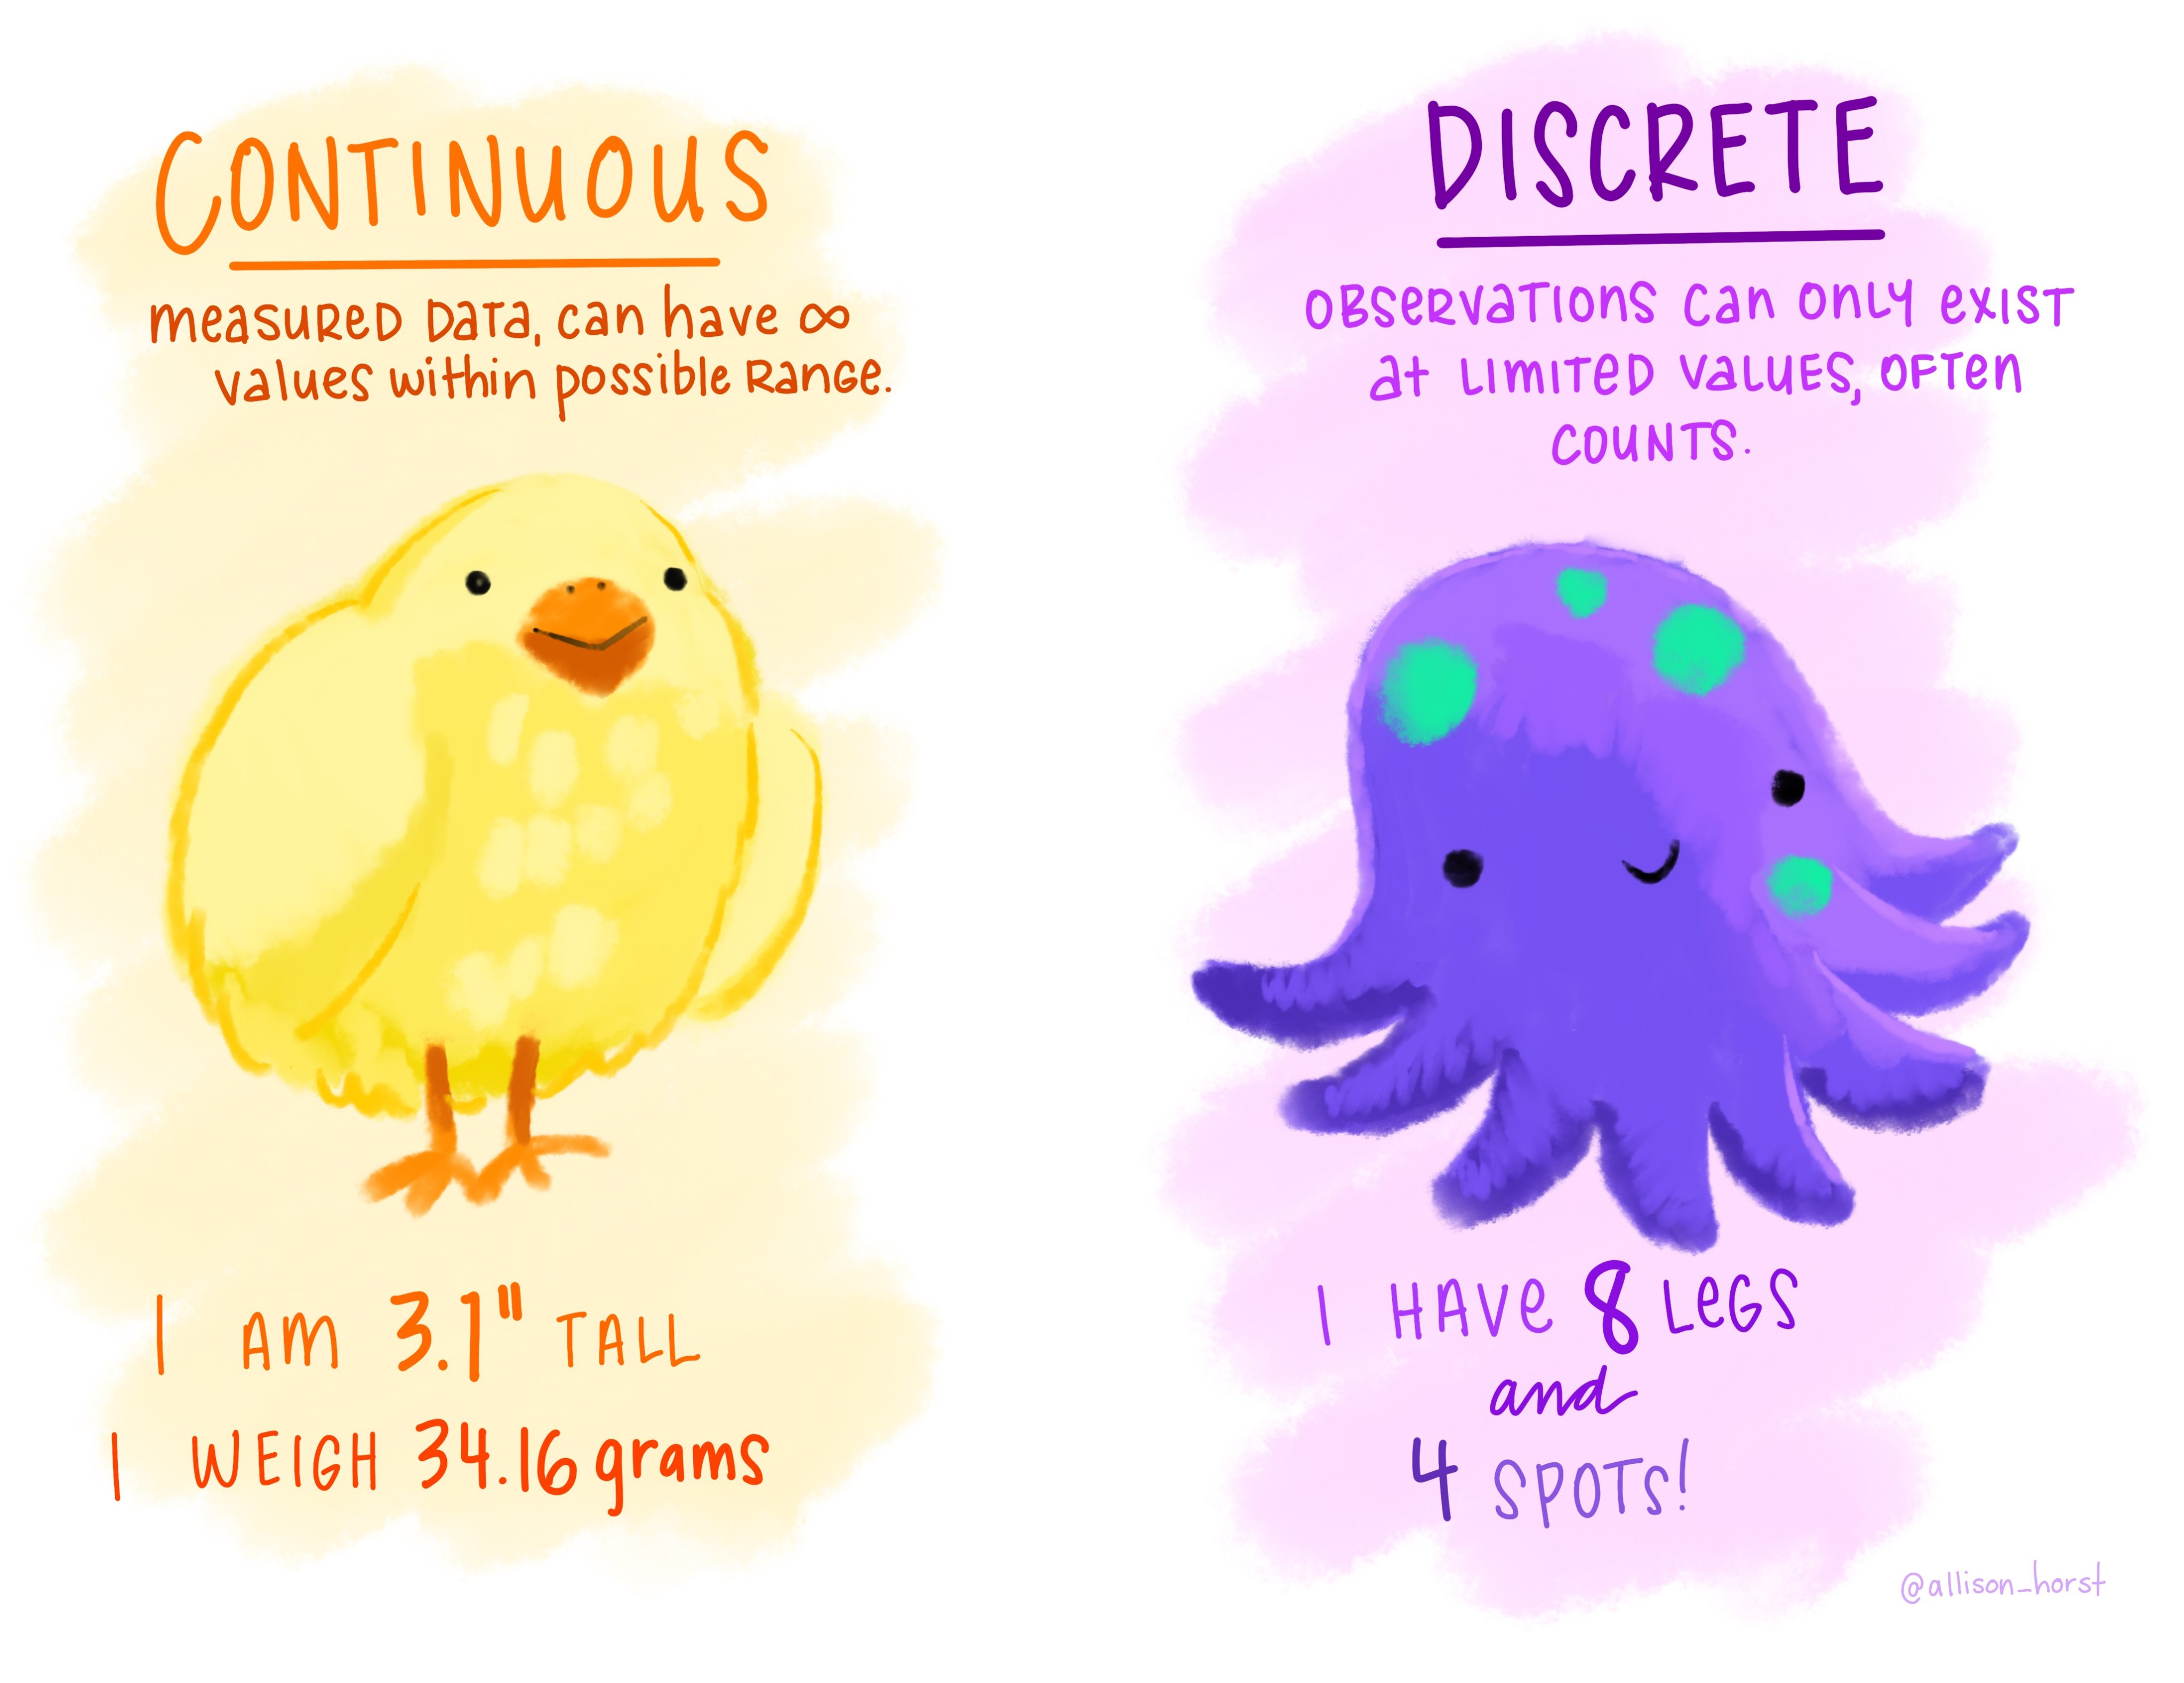
\includegraphics[width=\textwidth,height=0.75\textheight]{../images/cont_disc.jpg}

\href{https://twitter.com/allison_horst}{via @allison\_horst}

\end{frame}

\begin{frame}

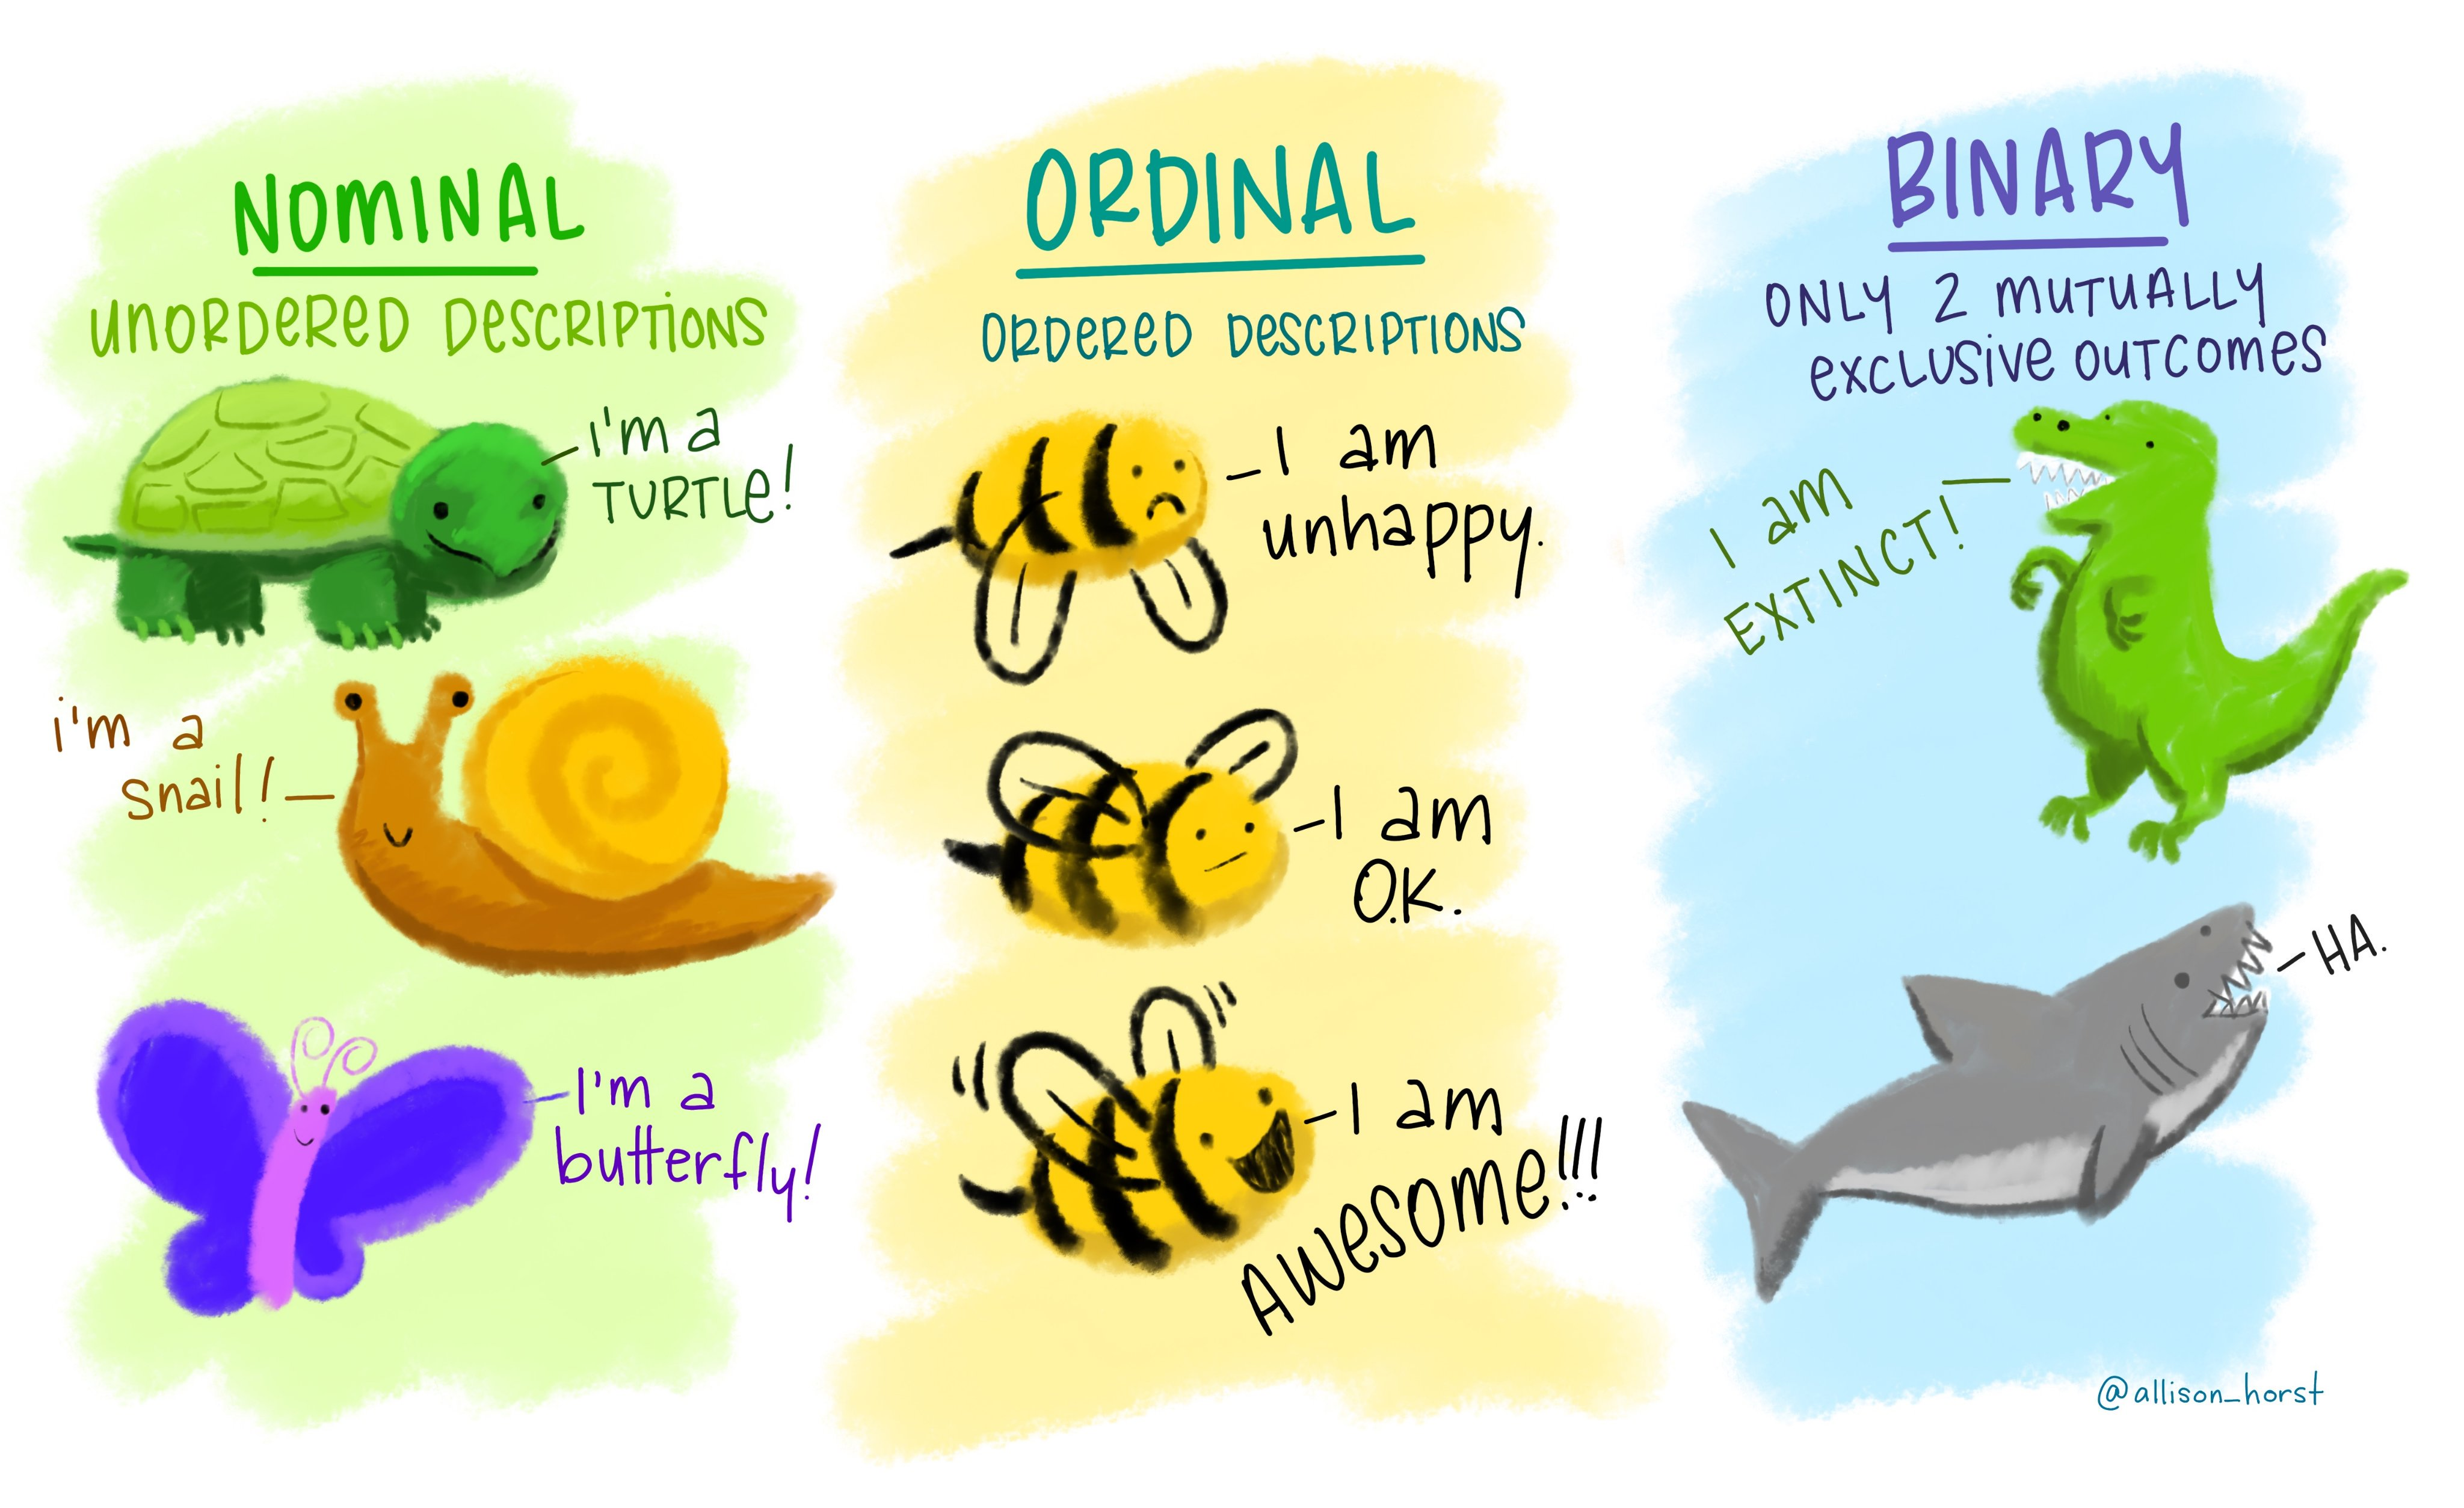
\includegraphics[width=\textwidth,height=0.75\textheight]{../images/nom_ord_bin.jpg}

\href{https://twitter.com/allison_horst}{via @allison\_horst}

\end{frame}

\begin{frame}

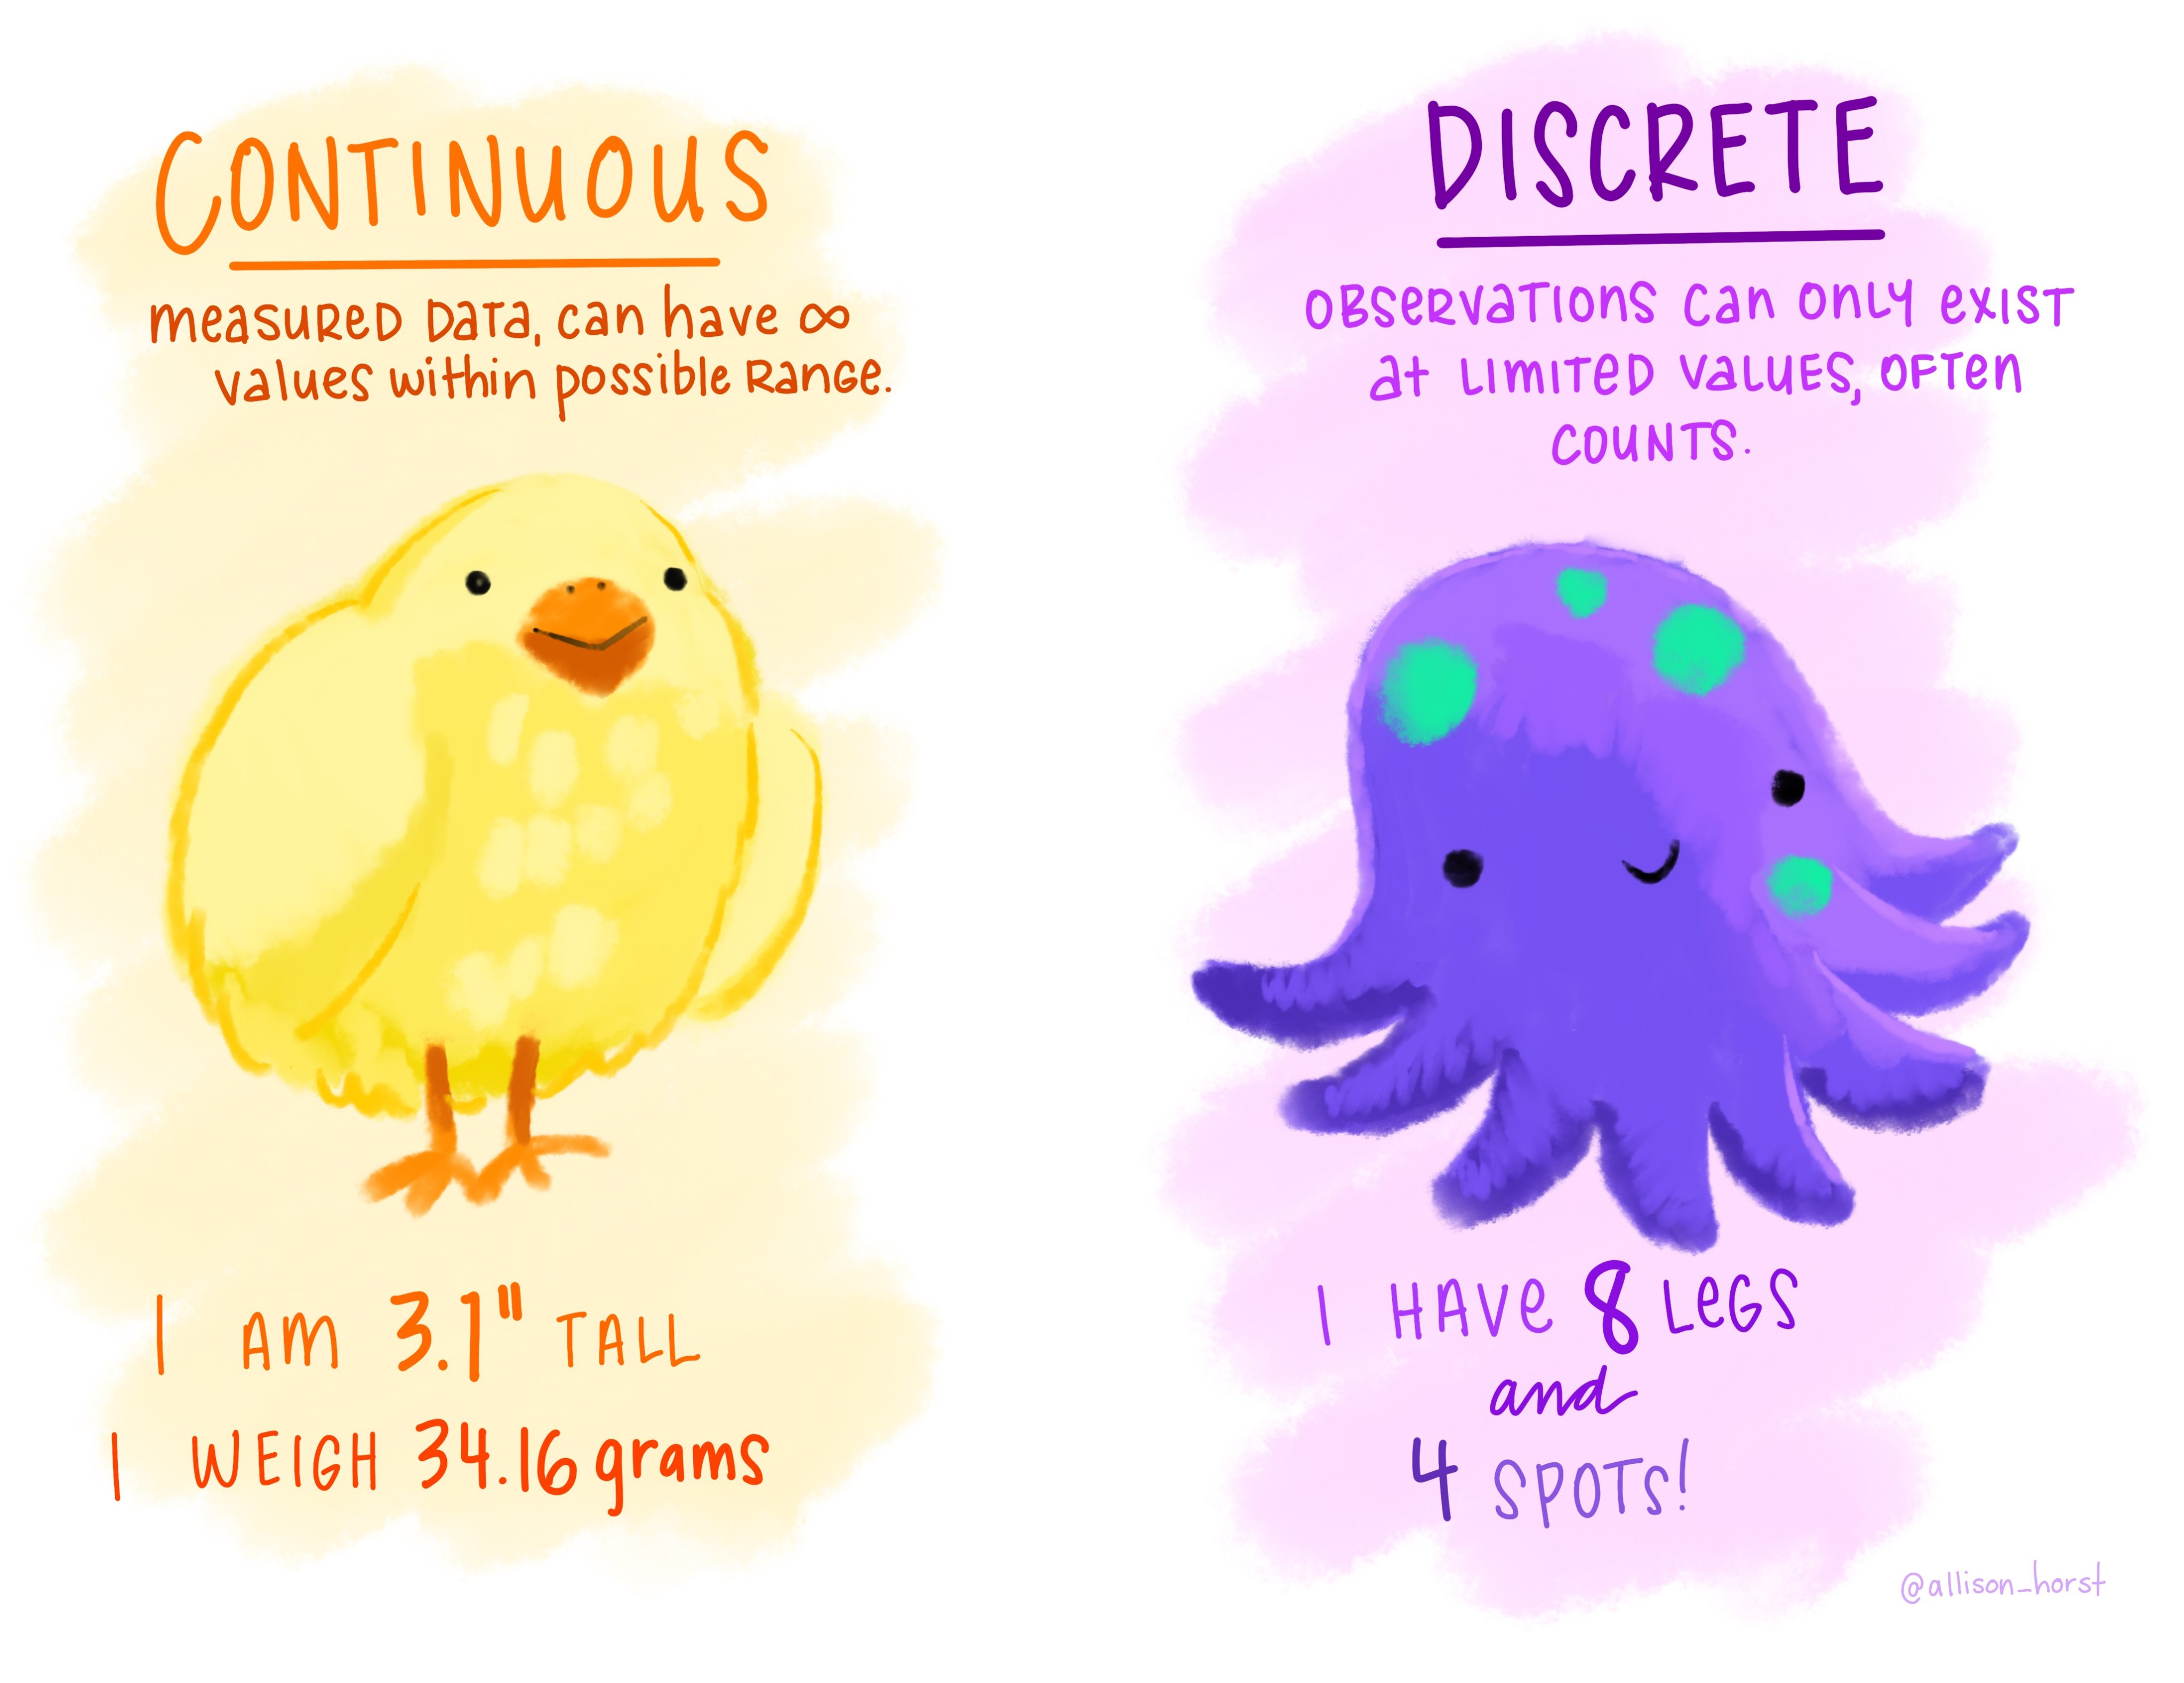
\includegraphics[width=\textwidth,height=0.4\textheight]{../images/cont_disc.jpg}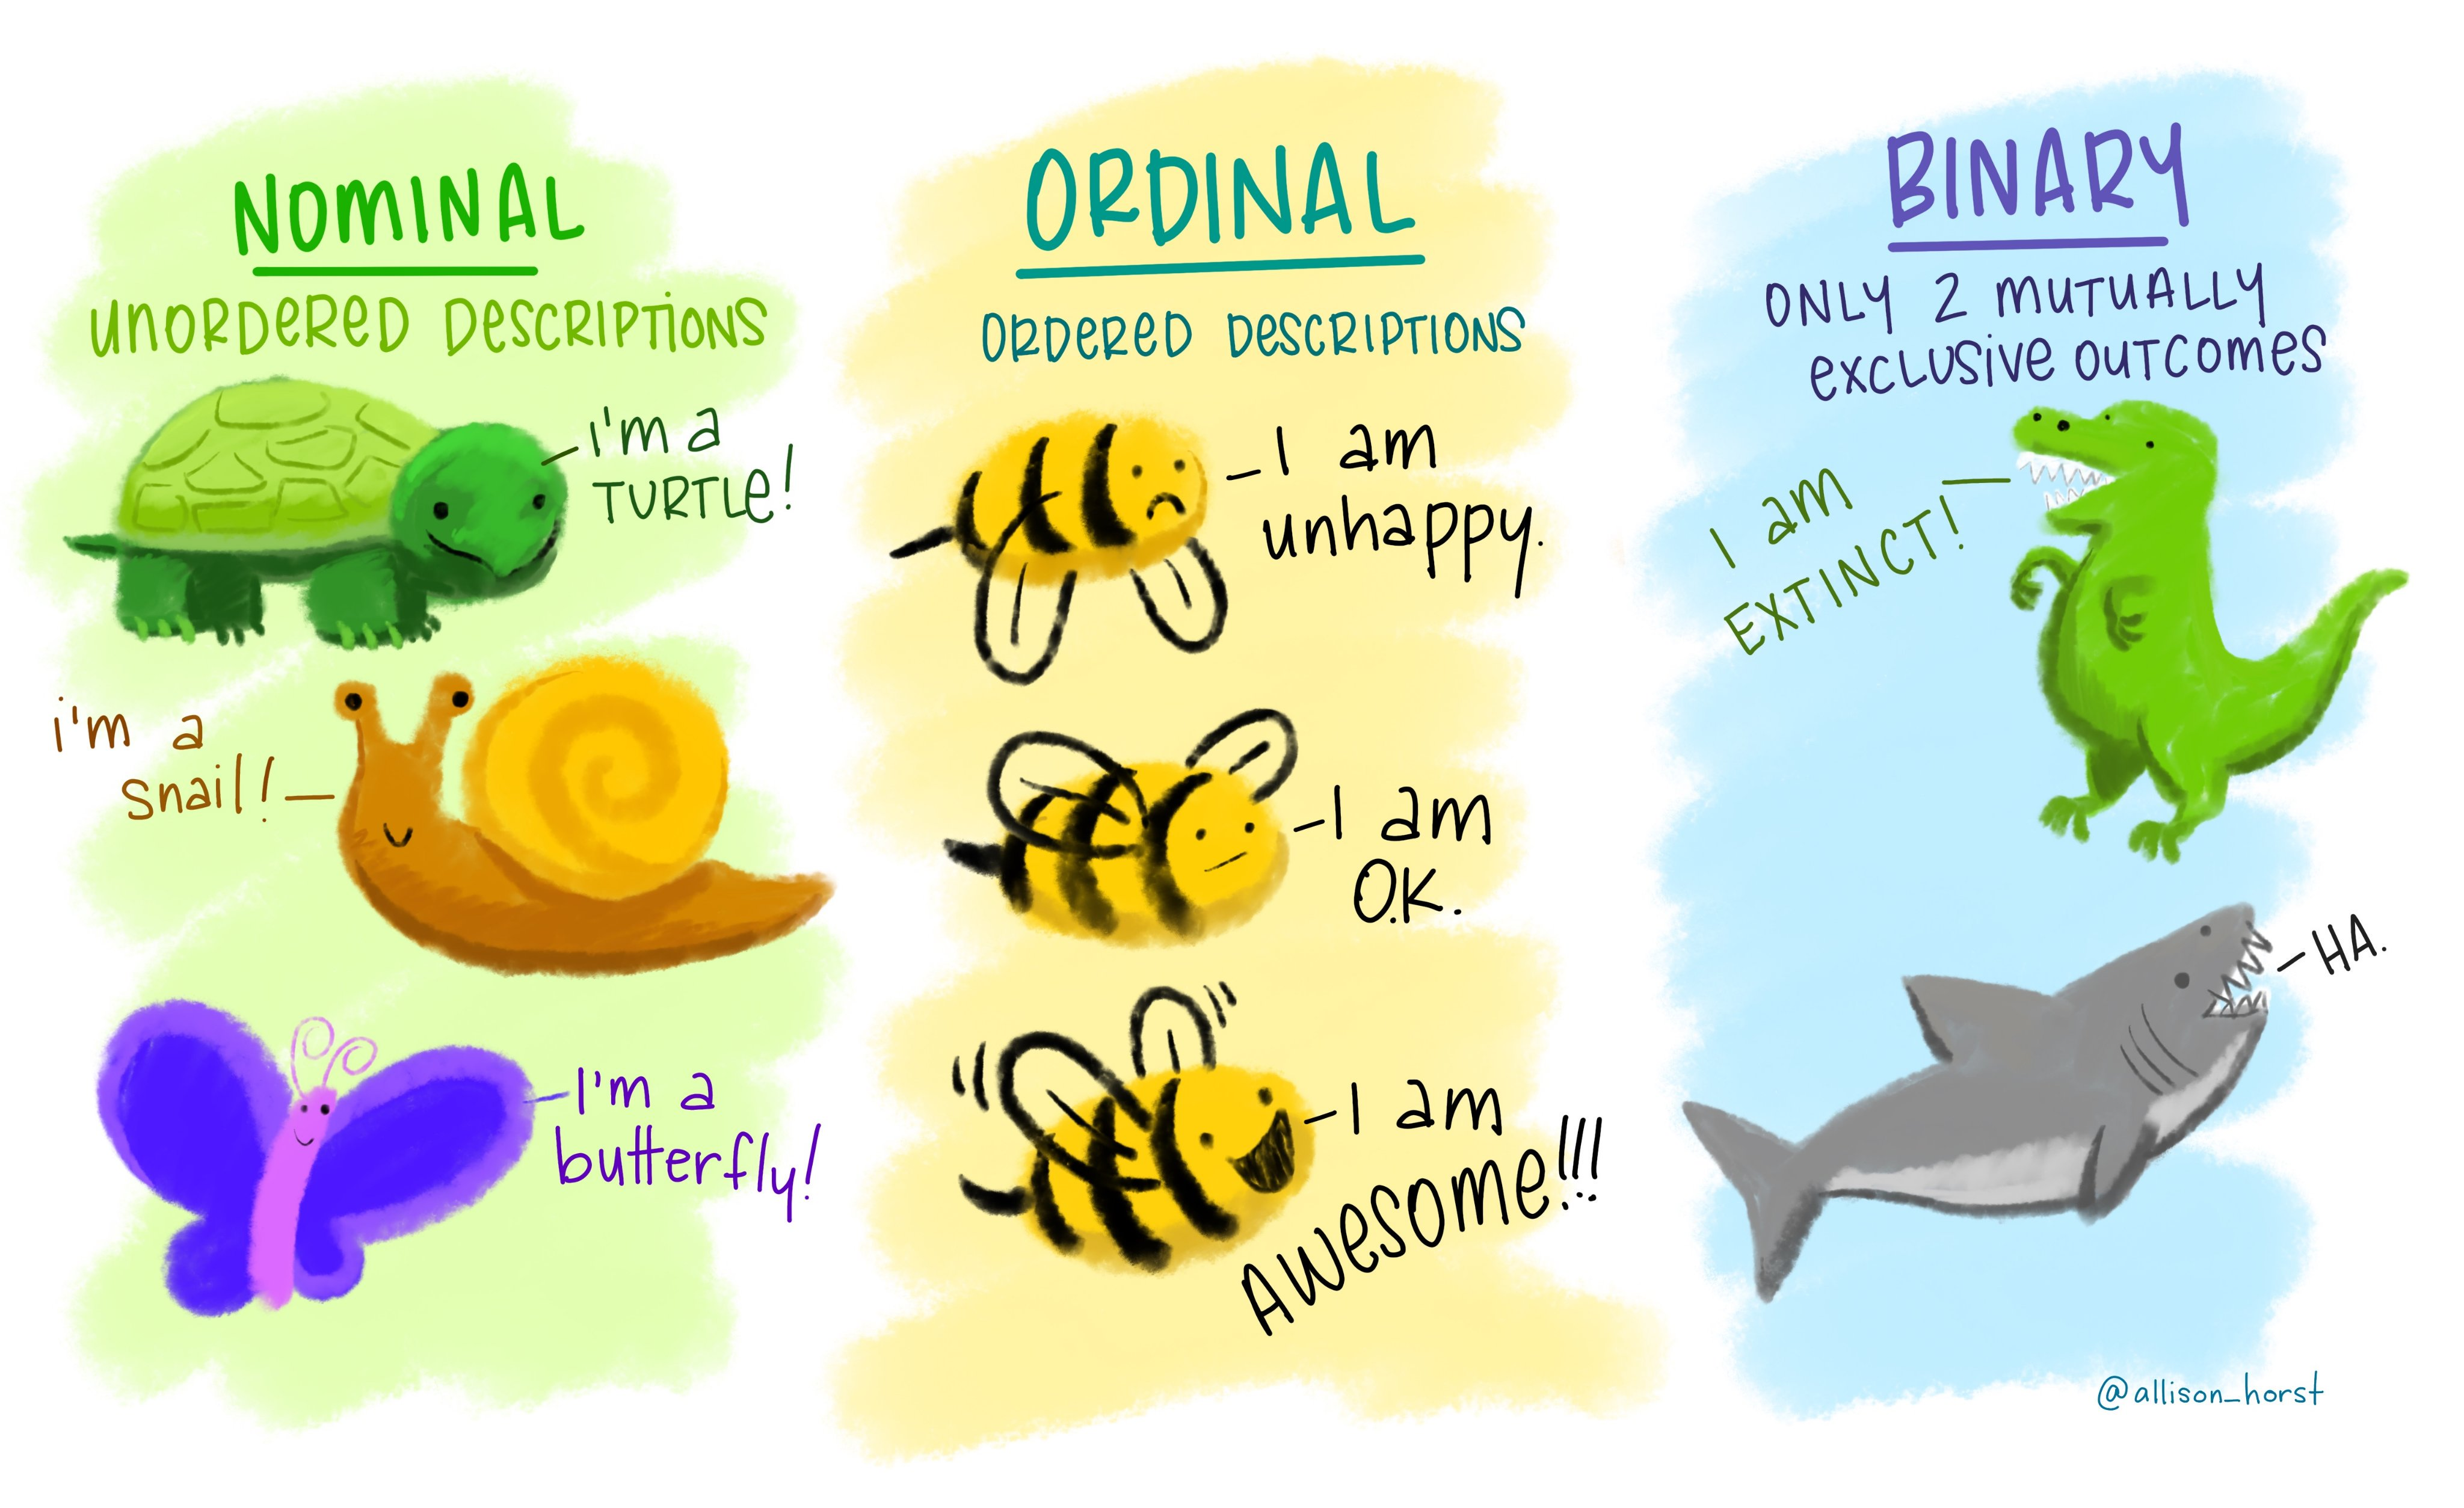
\includegraphics[width=\textwidth,height=0.4\textheight]{../images/nom_ord_bin.jpg}

\begin{itemize}[<+->]
\tightlist
\item
  What do we do with all of these in a PCA like way?
\item
  Some are \emph{very} difficult and effectively ignored

  \begin{itemize}[<+->]
  \tightlist
  \item
    We won't do that!
  \end{itemize}
\item
  See SS Steven's typology:
  \url{https://en.wikipedia.org/wiki/Level_of_measurement}
\end{itemize}

\end{frame}

\begin{frame}{Motivation \& Objectives}
\protect\hypertarget{motivation-objectives}{}

\begin{itemize}[<+->]
\tightlist
\item
  Not everything is a number

  \begin{itemize}[<+->]
  \tightlist
  \item
    Sometimes numbers aren't numbers!
  \end{itemize}
\item
  We need to recognize when this happens

  \begin{itemize}[<+->]
  \tightlist
  \item
    And know what to do
  \end{itemize}
\item
  Introduce CA, MCA, and tricks

  \begin{itemize}[<+->]
  \tightlist
  \item
    Leave you overwhelmed, but knowing that
  \item
    PCA is sometimes the most wrong approach
  \item
    CA \& MCA are suitably less wrong
  \end{itemize}
\end{itemize}

\end{frame}

\begin{frame}{Where to find everything}
\protect\hypertarget{where-to-find-everything}{}

\begin{itemize}[<+->]
\tightlist
\item
  Generally: \url{https://github.com/derekbeaton/workshops}
\item
  Today:
  \url{https://github.com/derekbeaton/Workshops/tree/master/Misc/CA_MCA}

  \begin{itemize}[<+->]
  \tightlist
  \item
    Built off of previous workshop
  \item
    Alzheimer's Disease Neuroimaging Initiative (ADNI) data
  \end{itemize}
\end{itemize}

\end{frame}

\begin{frame}{Overview}
\protect\hypertarget{overview}{}

\begin{itemize}[<+->]
\tightlist
\item
  Revisit PCA
\item
  Looking at some data
\item
  Simple correspondence analysis

  \begin{itemize}[<+->]
  \tightlist
  \item
    and many of its connections
  \end{itemize}
\item
  Multiple correspondence analysis

  \begin{itemize}[<+->]
  \tightlist
  \item
    generalizes CA (amongst many other things)
  \item
    and how to handle various data types
  \end{itemize}
\item
  A whole bunch of bonuses

  \begin{itemize}[<+->]
  \tightlist
  \item
    Robustness, PLS, Software
  \end{itemize}
\end{itemize}

\end{frame}

\hypertarget{revisting-pca}{%
\section{Revisting PCA}\label{revisting-pca}}

\begin{frame}{What is PCA for?}
\protect\hypertarget{what-is-pca-for}{}

\begin{itemize}[<+->]
\tightlist
\item
  When we can compute a covariance or correlation matrix
\item
  Break data into components

  \begin{itemize}[<+->]
  \tightlist
  \item
    Orthogonal
  \item
    Rank ordered
  \item
    Made of bits \& pieces of original measures
  \end{itemize}
\end{itemize}

\end{frame}

\hypertarget{some-data}{%
\section{Some data}\label{some-data}}

\begin{frame}{Diagnosis and education}
\protect\hypertarget{diagnosis-and-education}{}

\begin{table}[H]
\centering
\begin{tabular}{>{\em}lrrr}
\toprule
  & CN & Dementia & MCI\\
\midrule
ADV & 39 & 7 & 54\\
B & 57 & 17 & 75\\
B+ & 75 & 19 & 113\\
HS & 25 & 13 & 46\\
HS+ & 39 & 9 & 77\\
\bottomrule
\end{tabular}
\end{table}

\end{frame}

\begin{frame}

\begin{itemize}[<+->]
\tightlist
\item
  Given a table, and asked for a multivariate analysis
\item
  We do what we know: PCA
\end{itemize}

\end{frame}

\begin{frame}

\includegraphics{CA_MCA_Slides_files/figure-beamer/unnamed-chunk-1-1.pdf}

\end{frame}

\begin{frame}

\includegraphics{CA_MCA_Slides_files/figure-beamer/unnamed-chunk-2-1.pdf}

\end{frame}

\begin{frame}

\includegraphics{CA_MCA_Slides_files/figure-beamer/unnamed-chunk-3-1.pdf}

\end{frame}

\begin{frame}{What did we analyze?}
\protect\hypertarget{what-did-we-analyze}{}

\begin{table}[H]
\centering
\begin{tabular}{lrrr}
\toprule
  & CN & Dementia & MCI\\
\midrule
CN & 1.000 & 0.730 & 0.921\\
Dementia & 0.730 & 1.000 & 0.652\\
MCI & 0.921 & 0.652 & 1.000\\
\bottomrule
\end{tabular}
\end{table}

\end{frame}

\begin{frame}{What did PCA detect?}
\protect\hypertarget{what-did-pca-detect}{}

\begin{table}[H]
\centering
\begin{tabular}{>{\em}lrrr>{\bfseries\em}r}
\toprule
  & CN & Dementia & MCI & Row sums\\
\midrule
ADV & 39 & 7 & 54 & 100\\
B & 57 & 17 & 75 & 149\\
B+ & 75 & 19 & 113 & 207\\
HS & 25 & 13 & 46 & 84\\
HS+ & 39 & 9 & 77 & 125\\
\bottomrule
\end{tabular}
\end{table}

\end{frame}

\begin{frame}{Let's try something different!}
\protect\hypertarget{lets-try-something-different}{}

\end{frame}

\begin{frame}

\begin{table}[H]
\centering
\begin{tabular}{>{\em}lrrrrr}
\toprule
  & ADV & B & B+ & HS & HS+\\
\midrule
CN & 39 & 57 & 75 & 25 & 39\\
Dementia & 7 & 17 & 19 & 13 & 9\\
MCI & 54 & 75 & 113 & 46 & 77\\
\bottomrule
\end{tabular}
\end{table}

\end{frame}

\begin{frame}

\includegraphics{CA_MCA_Slides_files/figure-beamer/edu_dx_pca_2-1.pdf}

\end{frame}

\begin{frame}{What did PCA analyze?}
\protect\hypertarget{what-did-pca-analyze}{}

\begin{table}[H]
\centering
\begin{tabular}{lrrrrr}
\toprule
  & ADV & B & B+ & HS & HS+\\
\midrule
ADV & 1.000 & 1.000 & 0.995 & 0.935 & 0.963\\
B & 1.000 & 1.000 & 0.994 & 0.932 & 0.960\\
B+ & 0.995 & 0.994 & 1.000 & 0.965 & 0.984\\
HS & 0.935 & 0.932 & 0.965 & 1.000 & 0.996\\
HS+ & 0.963 & 0.960 & 0.984 & 0.996 & 1.000\\
\bottomrule
\end{tabular}
\end{table}

\end{frame}

\begin{frame}{What did PCA detect?}
\protect\hypertarget{what-did-pca-detect-1}{}

\begin{table}[H]
\centering
\begin{tabular}{>{\em}lrrrrr>{\bfseries\em}r}
\toprule
  & ADV & B & B+ & HS & HS+ & Row sums\\
\midrule
CN & 39 & 57 & 75 & 25 & 39 & 235\\
Dementia & 7 & 17 & 19 & 13 & 9 & 65\\
MCI & 54 & 75 & 113 & 46 & 77 & 365\\
\bottomrule
\end{tabular}
\end{table}

\end{frame}

\begin{frame}{What is PCA for?}
\protect\hypertarget{what-is-pca-for-1}{}

\begin{itemize}[<+->]
\tightlist
\item
  When we can compute a \emph{meaningful} covariance or correlation
  matrix
\end{itemize}

\end{frame}

\begin{frame}{Let's take another look}
\protect\hypertarget{lets-take-another-look}{}

\begin{table}[H]
\centering
\begin{tabular}{>{\em}lrrr>{\bfseries\em}r}
\toprule
  & CN & Dementia & MCI & Row sums\\
\midrule
ADV & 39 & 7 & 54 & 100\\
B & 57 & 17 & 75 & 149\\
B+ & 75 & 19 & 113 & 207\\
HS & 25 & 13 & 46 & 84\\
HS+ & 39 & 9 & 77 & 125\\
\addlinespace
\em{\textbf{Column sums}} & \em{\textbf{235}} & \em{\textbf{65}} & \em{\textbf{365}}\\
\bottomrule
\end{tabular}
\end{table}

\begin{itemize}[<+->]
\tightlist
\item
  Tell me things about this matrix
\item
  What kind of problem does this look like?
\end{itemize}

\end{frame}

\hypertarget{simple-correspondence-analysis}{%
\section{Simple correspondence
analysis}\label{simple-correspondence-analysis}}

\begin{frame}{What is CA?}
\protect\hypertarget{what-is-ca}{}

\begin{itemize}[<+->]
\tightlist
\item
  Initially: \emph{visualize contingency tables} (\textbf{a la PCA},
  factor analyses)

  \begin{itemize}[<+->]
  \tightlist
  \item
    Text (corpus) of philosphy, biblical passages, literature
  \item
    From Benzecri (1964) \& Escofier (1965)
  \item
    Fully developed by Escofier (1969)
  \end{itemize}
\item
  Explosion of the technique in France

  \begin{itemize}[<+->]
  \tightlist
  \item
    Across virtually every field (except psychology and neuroscience)
  \end{itemize}
\end{itemize}

\end{frame}

\begin{frame}{History}
\protect\hypertarget{history}{}

\begin{itemize}[<+->]
\tightlist
\item
  Hotelling (1933) \& Thurstone (1933)
\item
  Hirschfeld (1935) \& Horst (1935)
\item
  Guttman (1941)
\item
  Burt (1950)
\item
  And then Benzecri (1964) \& Escofier (1965)
\item
  Many more very important characters to re-discover CA
\end{itemize}

\end{frame}

\begin{frame}

\begin{itemize}[<+->]
\tightlist
\item
  See Lebart's History \& Prehistory of CA

  \begin{itemize}[<+->]
  \tightlist
  \item
    \url{http://www.dtmvic.com/doc/About_the_History_of_CA.pdf}
  \end{itemize}
\item
  And Beh \& Lombardo's series

  \begin{itemize}[<+->]
  \tightlist
  \item
    A geneaology of CA:
    \url{https://onlinelibrary.wiley.com/doi/abs/10.1111/j.1467-842X.2012.00676.x}
  \item
    A geneaology of CA 2:
    \url{http://siba-ese.unisalento.it/index.php/ejasa/article/view/19785}
  \end{itemize}
\end{itemize}

\end{frame}

\begin{frame}{We're diving in}
\protect\hypertarget{were-diving-in}{}

\end{frame}

\begin{frame}

\begin{table}[H]
\centering
\begin{tabular}{>{\em}lrrr}
\toprule
  & CN & Dementia & MCI\\
\midrule
ADV & 39 & 7 & 54\\
B & 57 & 17 & 75\\
B+ & 75 & 19 & 113\\
HS & 25 & 13 & 46\\
HS+ & 39 & 9 & 77\\
\bottomrule
\end{tabular}
\end{table}

\end{frame}

\begin{frame}

\includegraphics{CA_MCA_Slides_files/figure-beamer/show_ca_rows_1-1.pdf}

\end{frame}

\begin{frame}

\includegraphics{CA_MCA_Slides_files/figure-beamer/show_ca_cols_1-1.pdf}

\end{frame}

\begin{frame}

\includegraphics{CA_MCA_Slides_files/figure-beamer/show_ca_both_1-1.pdf}

\end{frame}

\begin{frame}

Want to see a cool trick?

\end{frame}

\begin{frame}

\begin{table}[H]
\centering
\begin{tabular}{>{\em}lrrr}
\toprule
  & CN & Dementia & MCI\\
\midrule
ADV & 39 & 7 & 54\\
B & 57 & 17 & 75\\
B+ & 75 & 19 & 113\\
HS & 25 & 13 & 46\\
HS+ & 39 & 9 & 77\\
\bottomrule
\end{tabular}
\end{table}

\end{frame}

\begin{frame}

\begin{table}[H]
\centering
\begin{tabular}{>{\em}lrrrrr}
\toprule
  & ADV & B & B+ & HS & HS+\\
\midrule
CN & 39 & 57 & 75 & 25 & 39\\
Dementia & 7 & 17 & 19 & 13 & 9\\
MCI & 54 & 75 & 113 & 46 & 77\\
\bottomrule
\end{tabular}
\end{table}

\end{frame}

\begin{frame}

\includegraphics{CA_MCA_Slides_files/figure-beamer/ca_results_transponse-1.pdf}

\end{frame}

\begin{frame}{How did that happen?}
\protect\hypertarget{how-did-that-happen}{}

\begin{table}[t]

\caption{\label{tab:edu_dx_chi2}Data}
\centering
\begin{tabular}{>{\em}lrrr}
\toprule
  & CN & Dementia & MCI\\
\midrule
ADV & 39 & 7 & 54\\
B & 57 & 17 & 75\\
B+ & 75 & 19 & 113\\
HS & 25 & 13 & 46\\
HS+ & 39 & 9 & 77\\
\bottomrule
\end{tabular}
\end{table}

\end{frame}

\begin{frame}

\begin{table}[t]

\caption{\label{tab:edu_dx_chi2_o}Observed probabilites}
\centering
\begin{tabular}{>{\em}lrrr}
\toprule
  & CN & Dementia & MCI\\
\midrule
ADV & 0.059 & 0.011 & 0.081\\
B & 0.086 & 0.026 & 0.113\\
B+ & 0.113 & 0.029 & 0.170\\
HS & 0.038 & 0.020 & 0.069\\
HS+ & 0.059 & 0.014 & 0.116\\
\bottomrule
\end{tabular}
\end{table}

\end{frame}

\begin{frame}

\begin{table}[t]

\caption{\label{tab:edu_dx_chi2_osums}Observed probabilites and margins}
\centering
\begin{tabular}{>{\em}lrrr>{\bfseries\em}r}
\toprule
  & CN & Dementia & MCI & Row sums\\
\midrule
ADV & 0.059 & 0.011 & 0.081 & 0.150\\
B & 0.086 & 0.026 & 0.113 & 0.224\\
B+ & 0.113 & 0.029 & 0.170 & 0.311\\
HS & 0.038 & 0.020 & 0.069 & 0.126\\
HS+ & 0.059 & 0.014 & 0.116 & 0.188\\
\addlinespace
\em{\textbf{Column sums}} & \em{\textbf{0.353}} & \em{\textbf{0.098}} & \em{\textbf{0.549}}\\
\bottomrule
\end{tabular}
\end{table}

\end{frame}

\begin{frame}

\begin{table}[t]

\caption{\label{tab:edu_dx_chi2_e}Expected probabilites and margins}
\centering
\begin{tabular}{>{\em}lrrr>{\bfseries\em}r}
\toprule
  & CN & Dementia & MCI & Row sums\\
\midrule
ADV & 0.053 & 0.015 & 0.083 & 0.150\\
B & 0.079 & 0.022 & 0.123 & 0.224\\
B+ & 0.110 & 0.030 & 0.171 & 0.311\\
HS & 0.045 & 0.012 & 0.069 & 0.126\\
HS+ & 0.066 & 0.018 & 0.103 & 0.188\\
\addlinespace
\em{\textbf{Column sums}} & \em{\textbf{0.353}} & \em{\textbf{0.098}} & \em{\textbf{0.549}}\\
\bottomrule
\end{tabular}
\end{table}

\end{frame}

\begin{frame}

\begin{table}[t]

\caption{\label{tab:edu_dx_chi2_z}Deviations: Observed - Expected}
\centering
\begin{tabular}{>{\em}lrrr}
\toprule
  & CN & Dementia & MCI\\
\midrule
ADV & 0.006 & -0.004 & -0.001\\
B & 0.007 & 0.004 & -0.010\\
B+ & 0.003 & -0.002 & -0.001\\
HS & -0.007 & 0.007 & 0.000\\
HS+ & -0.008 & -0.005 & 0.013\\
\bottomrule
\end{tabular}
\end{table}

\end{frame}

\begin{frame}

\begin{table}[t]

\caption{\label{tab:edu_dx_chi2_rowconstraints}Row constraints (inverse row margins)}
\centering
\begin{tabular}{>{\em}lrrrrr}
\toprule
  & ADV & B & B+ & HS & HS+\\
\midrule
ADV & 6.65 & 0.000 & 0.000 & 0.000 & 0.00\\
B & 0.00 & 4.463 & 0.000 & 0.000 & 0.00\\
B+ & 0.00 & 0.000 & 3.213 & 0.000 & 0.00\\
HS & 0.00 & 0.000 & 0.000 & 7.917 & 0.00\\
HS+ & 0.00 & 0.000 & 0.000 & 0.000 & 5.32\\
\bottomrule
\end{tabular}
\end{table}

\end{frame}

\begin{frame}

\begin{table}[t]

\caption{\label{tab:edu_dx_chi2_colconstraints}Column constraints (inverse column margins)}
\centering
\begin{tabular}{>{\em}lrrr}
\toprule
  & CN & Dementia & MCI\\
\midrule
CN & 2.83 & 0.000 & 0.000\\
Dementia & 0.00 & 10.231 & 0.000\\
MCI & 0.00 & 0.000 & 1.822\\
\bottomrule
\end{tabular}
\end{table}

\end{frame}

\begin{frame}{What CA needs}
\protect\hypertarget{what-ca-needs}{}

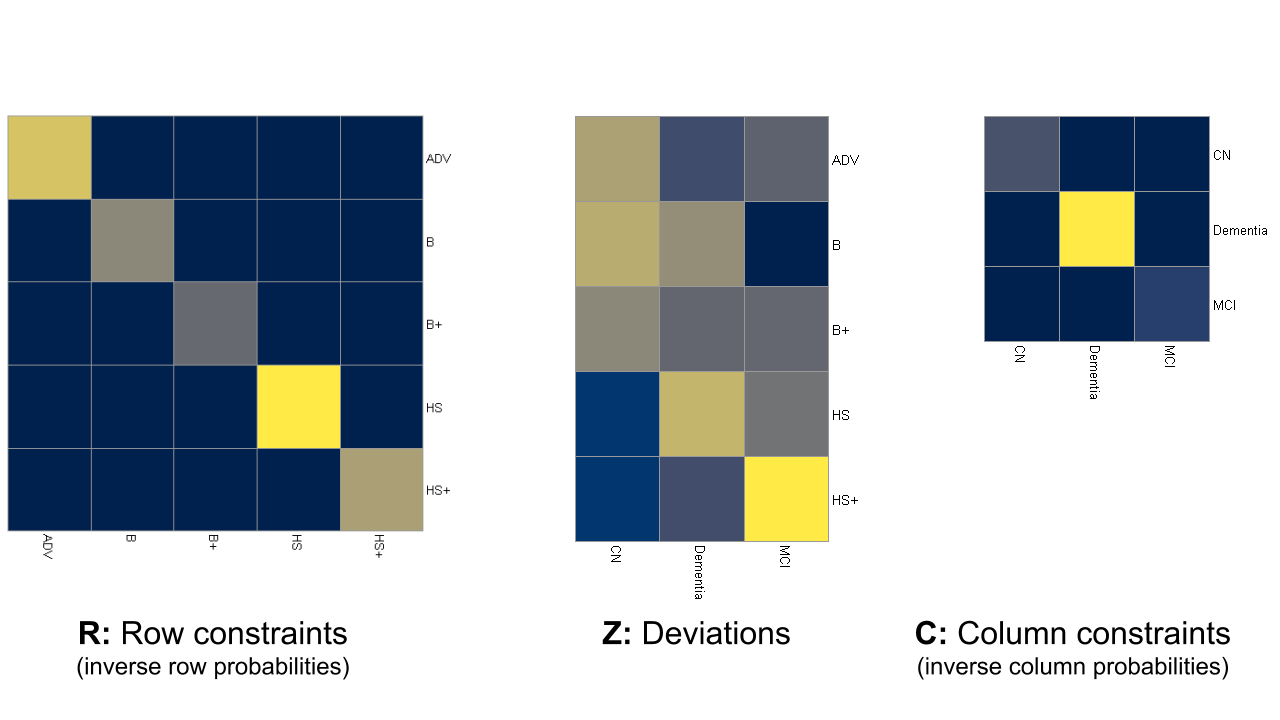
\includegraphics{../images/CA_matrices.png}

\end{frame}

\begin{frame}

\begin{itemize}[<+->]
\tightlist
\item
  GSVD(\(\mathbf{R}\), \(\mathbf{X}\), \(\mathbf{C}\))
\item
  Uses but generalizes the SVD

  \begin{itemize}[<+->]
  \tightlist
  \item
    Uses row \& column weights (constraints)
  \end{itemize}
\item
  Gives back

  \begin{itemize}[<+->]
  \tightlist
  \item
    Component (factor) scores
  \item
    Eigenvalues, singular values, \& singular vectors
  \item
    \emph{Generalized} singular vectors
  \end{itemize}
\end{itemize}

\end{frame}

\begin{frame}{What we really decompose}
\protect\hypertarget{what-we-really-decompose}{}

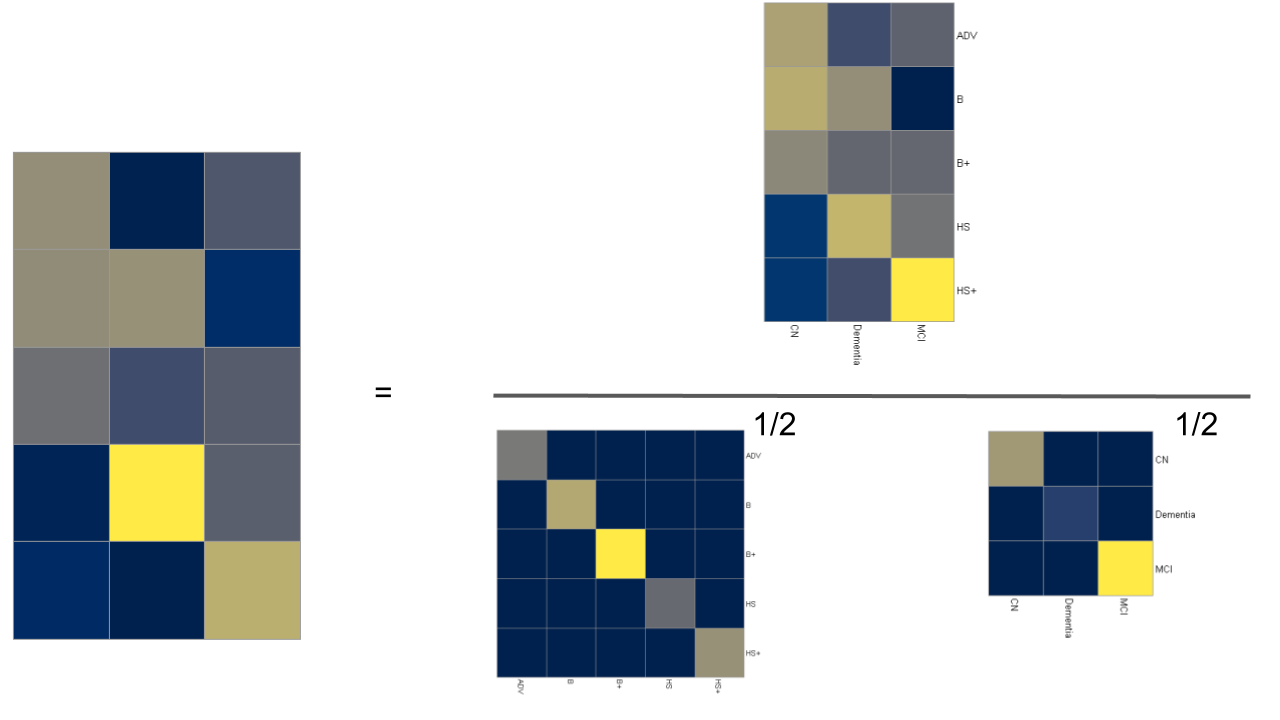
\includegraphics{../images/Deviations_Over_2.png}

\end{frame}

\begin{frame}{What we really decompose}
\protect\hypertarget{what-we-really-decompose-1}{}

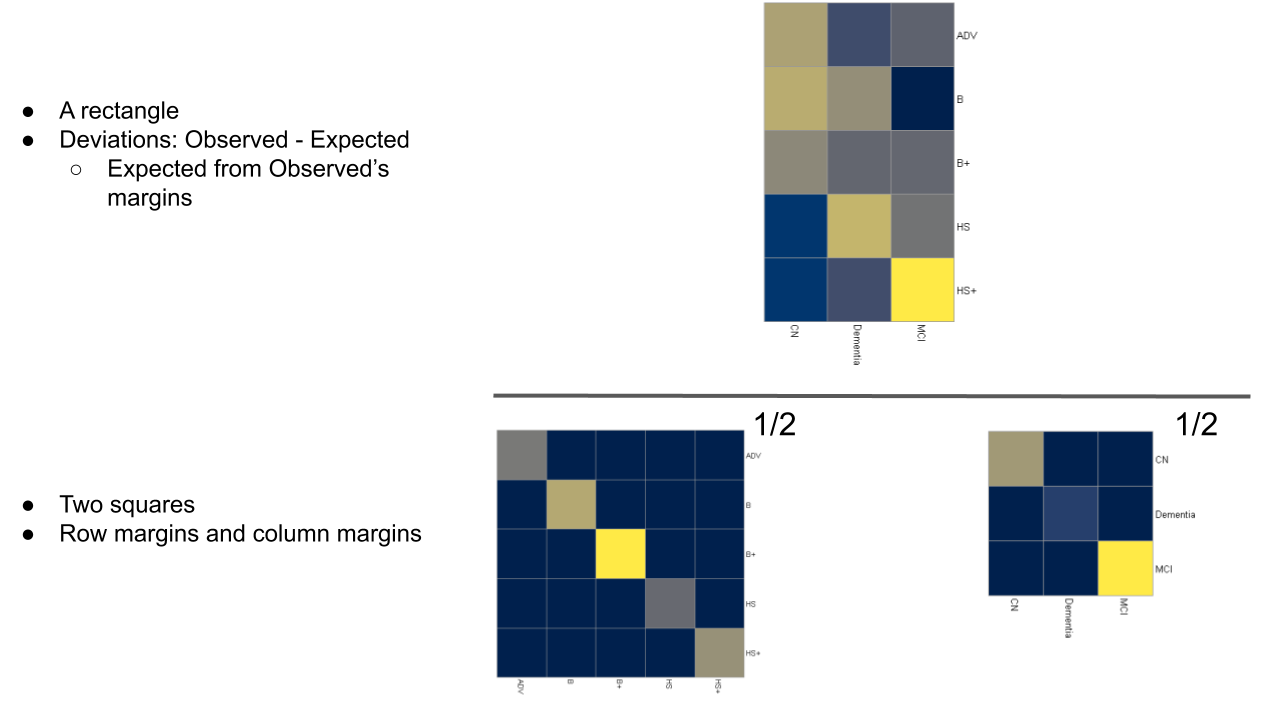
\includegraphics{../images/Deviations_Over.png}

\end{frame}

\begin{frame}

\begingroup\Huge

\begin{equation*}
\frac{\mathbf{Z}}{\mathbf{R}^{\frac{1}{2}}\mathbf{C}^{\frac{1}{2}}}
\end{equation*} \endgroup

\end{frame}

\begin{frame}

\begingroup\Huge

\begin{equation*}
\frac{(\mathbf{O} - \mathbf{E})}{\mathbf{E}^{\frac{1}{2}}}
\end{equation*} \endgroup

\end{frame}

\begin{frame}

\begingroup\Huge

\begin{equation*}
\chi^2 = \sum{\frac{(\mathbf{O} - \mathbf{E})^2}{\mathbf{E}}}
\end{equation*} \endgroup

\end{frame}

\begin{frame}[fragile]{CA's secrets}
\protect\hypertarget{cas-secrets}{}

\begin{Shaded}
\begin{Highlighting}[]
\NormalTok{EDU <-}\StringTok{ }\NormalTok{amerge_subset}\OperatorTok{$}\NormalTok{PTEDUCAT}
\NormalTok{DX <-}\StringTok{ }\NormalTok{amerge_subset}\OperatorTok{$}\NormalTok{DX}
\NormalTok{edu_dx_table <-}\StringTok{ }\KeywordTok{table}\NormalTok{(EDU, DX)}

\KeywordTok{chisq.test}\NormalTok{(edu_dx_table)}
\end{Highlighting}
\end{Shaded}

\begin{verbatim}
## 
##  Pearson's Chi-squared test
## 
## data:  edu_dx_table
## X-squared = 8.648, df = 8, p-value = 0.3729
\end{verbatim}

\begin{Shaded}
\begin{Highlighting}[]
\NormalTok{edu_dx_ca <-}\StringTok{ }\KeywordTok{epCA}\NormalTok{(edu_dx_table, }\DataTypeTok{graphs =}\NormalTok{ F)}
\KeywordTok{sum}\NormalTok{(edu_dx_ca}\OperatorTok{$}\NormalTok{ExPosition.Data}\OperatorTok{$}\NormalTok{eigs) }\OperatorTok{*}\StringTok{ }\KeywordTok{sum}\NormalTok{(edu_dx_table)}
\end{Highlighting}
\end{Shaded}

\begin{verbatim}
## [1] 8.647979
\end{verbatim}

\end{frame}

\begin{frame}

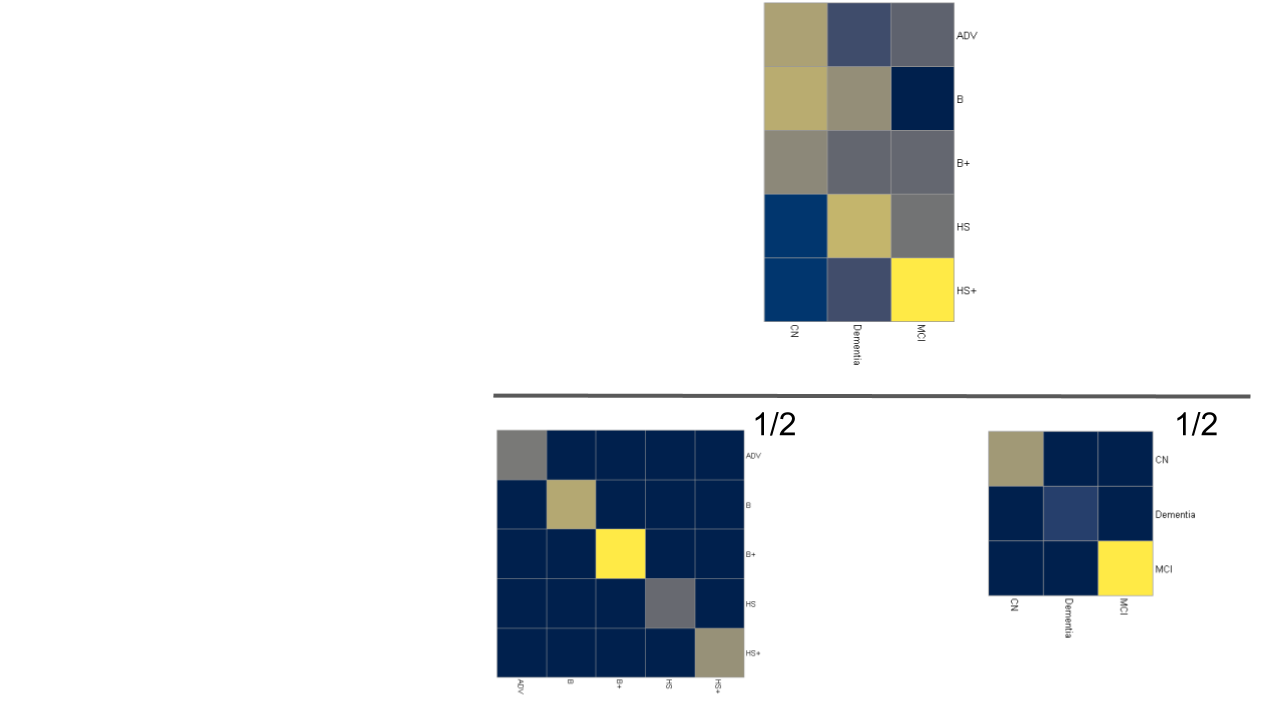
\includegraphics{../images/Deviations_Over_Familiar.png}

Besides \(\chi^2\) this looks really familiar. What else are rectangles
over squares?

\end{frame}

\begin{frame}

\begingroup\Huge

\begin{equation*}
r = \frac{cov(\mathbf{x},\mathbf{y})}{\sigma_{\mathbf{x}} \times \sigma_{\mathbf{y}}}
\end{equation*} \endgroup

\end{frame}

\begin{frame}{More of CA's secrets}
\protect\hypertarget{more-of-cas-secrets}{}

\begin{itemize}[<+->]
\tightlist
\item
  CA generalizes canonical correlation analysis (CCA)
\item
  CA is the CCA between two \emph{nominal} tables
\item
  How do we create a contingency table?
\end{itemize}

\end{frame}

\begin{frame}{Nominal data}
\protect\hypertarget{nominal-data}{}

\begin{center}
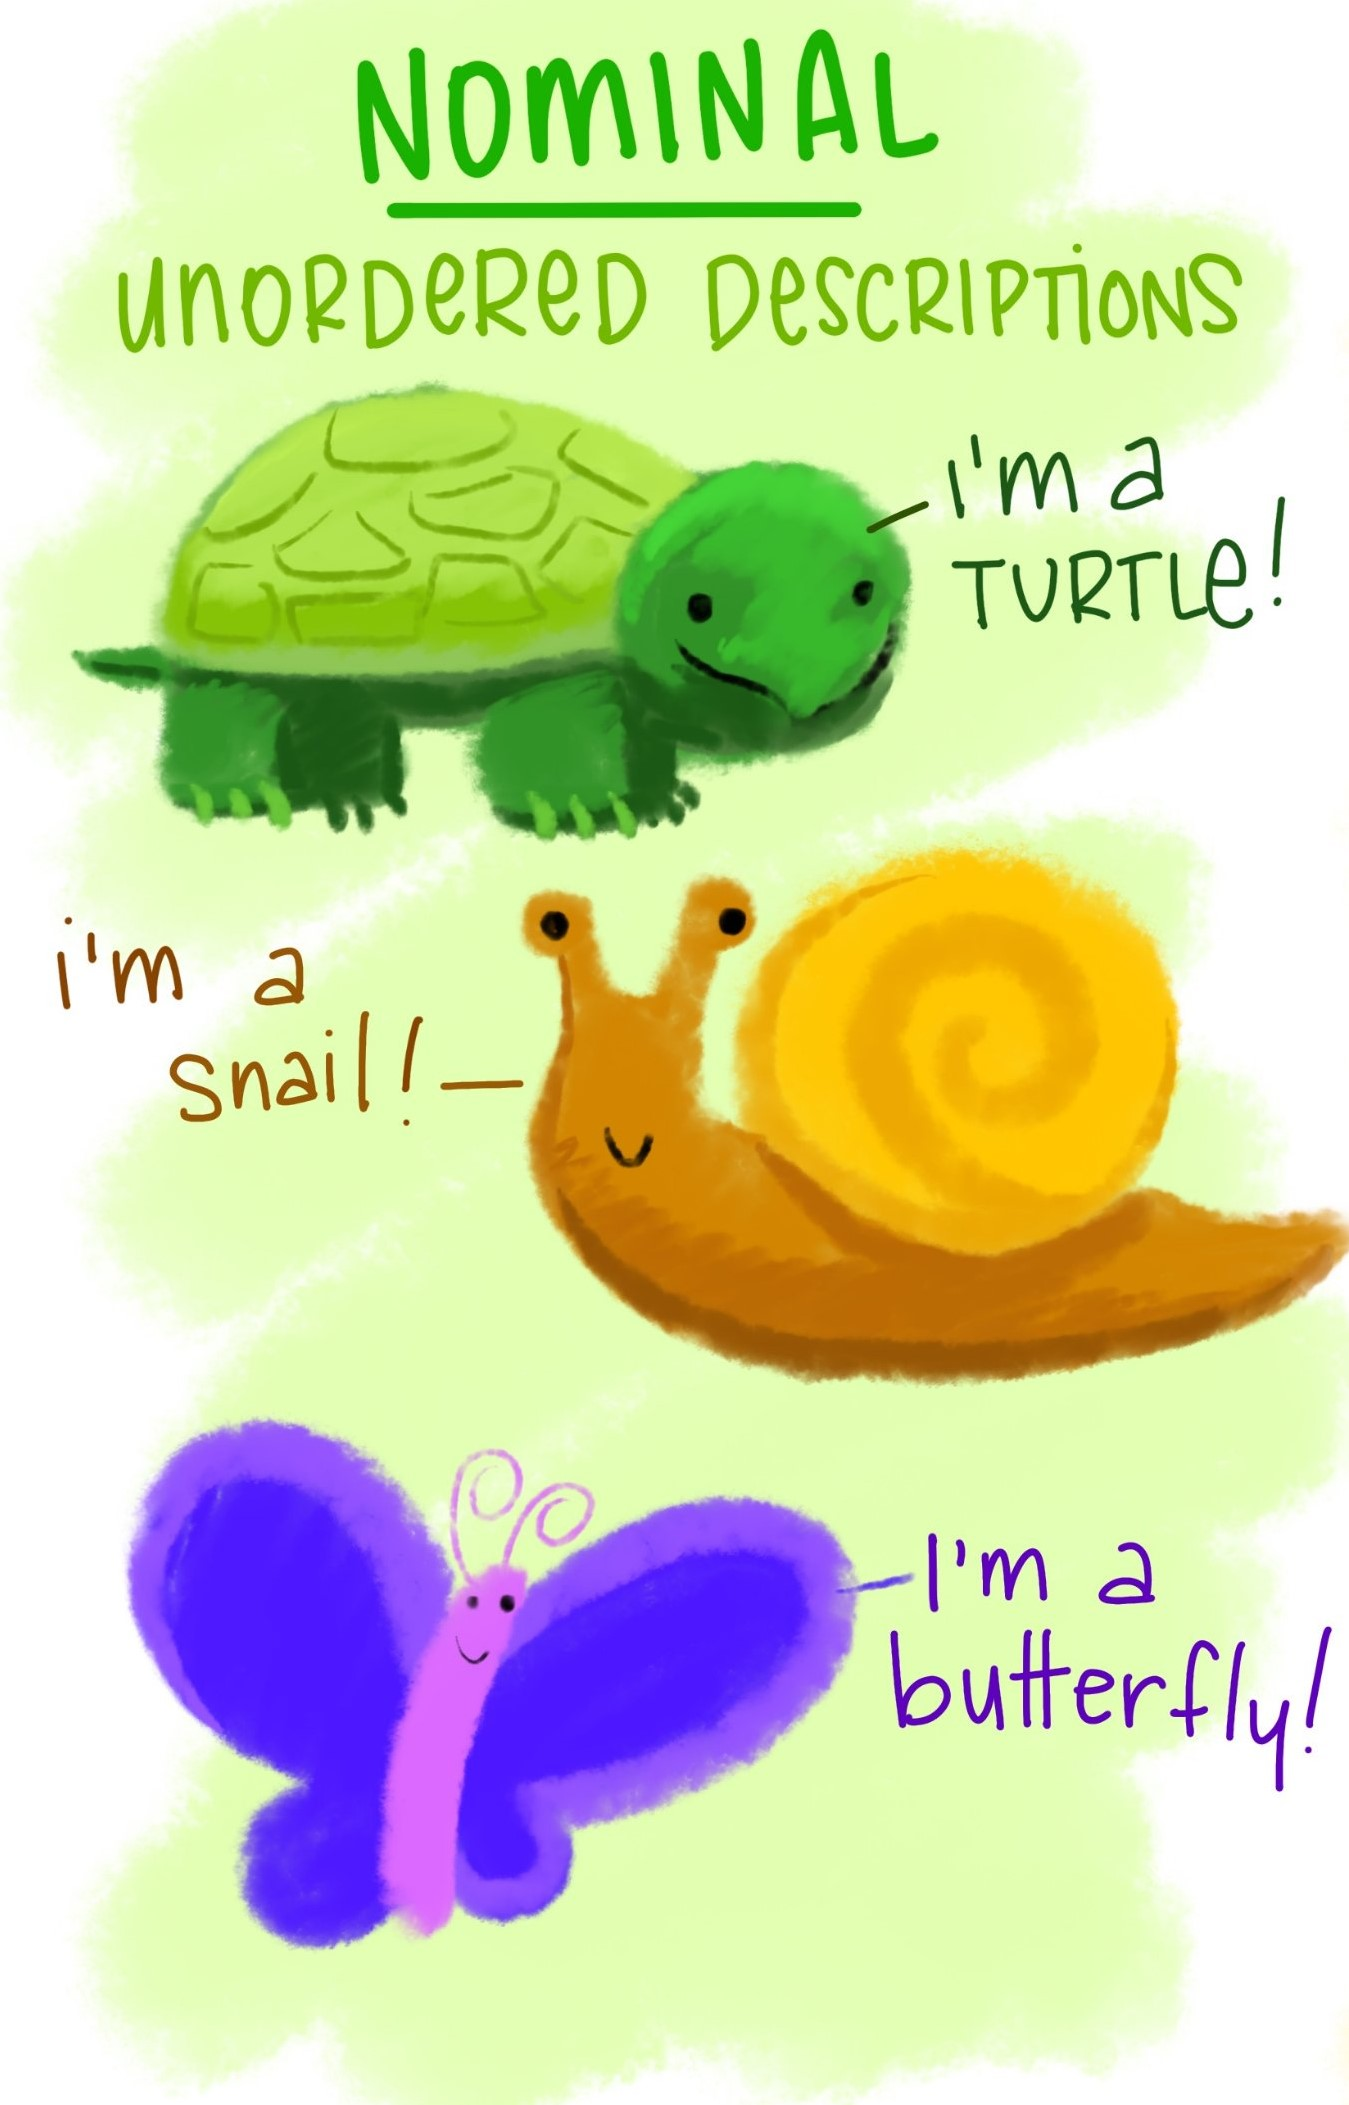
\includegraphics{../images/nom_copy.jpg}
\end{center}

\end{frame}

\begin{frame}

\includegraphics{CA_MCA_Slides_files/figure-beamer/show_nominal_1-1.pdf}

\end{frame}

\begin{frame}

\includegraphics{CA_MCA_Slides_files/figure-beamer/show_nominal_2-1.pdf}

\end{frame}

\begin{frame}

\includegraphics{CA_MCA_Slides_files/figure-beamer/show_nominal_3-1.pdf}
How to analyze this \emph{on its own}?

\end{frame}

\begin{frame}{How to analyze nominal data?}
\protect\hypertarget{how-to-analyze-nominal-data}{}

\begin{itemize}[<+->]
\tightlist
\item
  ``coding categorical variables with the indicator matrix of dummy
  variables and considering them as Gaussian, for instance, is almost a
  crime.'' in \emph{Jan de Leeuw and the French School of Data Analysis}
  (Husson, Josse, Saporta)
\item
  We \emph{could} perform PCA on nominal data, but what would we get?
\end{itemize}

\end{frame}

\begin{frame}

\includegraphics{CA_MCA_Slides_files/figure-beamer/crimes-1.pdf}

\end{frame}

\hypertarget{multiple-correspondence-analysis}{%
\section{Multiple correspondence
analysis}\label{multiple-correspondence-analysis}}

\begin{frame}{Multiple correspondence analysis}
\protect\hypertarget{multiple-correspondence-analysis-1}{}

\begin{itemize}[<+->]
\tightlist
\item
  Two perspectives:

  \begin{itemize}[<+->]
  \tightlist
  \item
    \emph{Weighted} PCA for nominal data
  \item
    Generalized CA for N-way contingency tables
  \end{itemize}
\item
  So much more than nominal
\end{itemize}

\end{frame}

\begin{frame}{We're diving in}
\protect\hypertarget{were-diving-in-1}{}

\includegraphics{CA_MCA_Slides_files/figure-beamer/show_nom-1.pdf}

This is the kind of table we're analyzing. It has \(N = 665\).

\end{frame}

\begin{frame}

\includegraphics{CA_MCA_Slides_files/figure-beamer/unnamed-chunk-5-1.pdf}

\end{frame}

\begin{frame}

\includegraphics{CA_MCA_Slides_files/figure-beamer/unnamed-chunk-6-1.pdf}

\end{frame}

\begin{frame}

\includegraphics{CA_MCA_Slides_files/figure-beamer/unnamed-chunk-7-1.pdf}

\end{frame}

\begin{frame}

\includegraphics{CA_MCA_Slides_files/figure-beamer/unnamed-chunk-8-1.pdf}

\end{frame}

\begin{frame}

\includegraphics{CA_MCA_Slides_files/figure-beamer/unnamed-chunk-9-1.pdf}

\end{frame}

\begin{frame}

\includegraphics{CA_MCA_Slides_files/figure-beamer/unnamed-chunk-10-1.pdf}

\end{frame}

\begin{frame}{CA \& MCA Magic!}
\protect\hypertarget{ca-mca-magic}{}

\includegraphics{CA_MCA_Slides_files/figure-beamer/show_nom_and_contingency-1.pdf}

Same technique on two \emph{different} tables: same result

\end{frame}

\begin{frame}{Scaling up}
\protect\hypertarget{scaling-up}{}

\begin{itemize}[<+->]
\tightlist
\item
  Let's bring in ApoE
\item
  It has 3 levels: 0 copy, 1 copy, 2 copies
\end{itemize}

\end{frame}

\begin{frame}

\includegraphics{CA_MCA_Slides_files/figure-beamer/new_cat_mat_0-1.pdf}

\end{frame}

\begin{frame}

\includegraphics{CA_MCA_Slides_files/figure-beamer/unnamed-chunk-11-1.pdf}

\end{frame}

\begin{frame}

\includegraphics{CA_MCA_Slides_files/figure-beamer/unnamed-chunk-12-1.pdf}

\end{frame}

\begin{frame}

\includegraphics{CA_MCA_Slides_files/figure-beamer/unnamed-chunk-13-1.pdf}

\end{frame}

\begin{frame}{Crisp vs.~fuzzy coding}
\protect\hypertarget{crisp-vs.-fuzzy-coding}{}

\includegraphics{CA_MCA_Slides_files/figure-beamer/show_crisp-1.pdf}

\end{frame}

\begin{frame}{Crisp vs.~fuzzy coding}
\protect\hypertarget{crisp-vs.-fuzzy-coding-1}{}

\includegraphics{CA_MCA_Slides_files/figure-beamer/show_fuzzy-1.pdf}

\end{frame}

\begin{frame}{Our first fuzzy friend}
\protect\hypertarget{our-first-fuzzy-friend}{}

\begin{center}
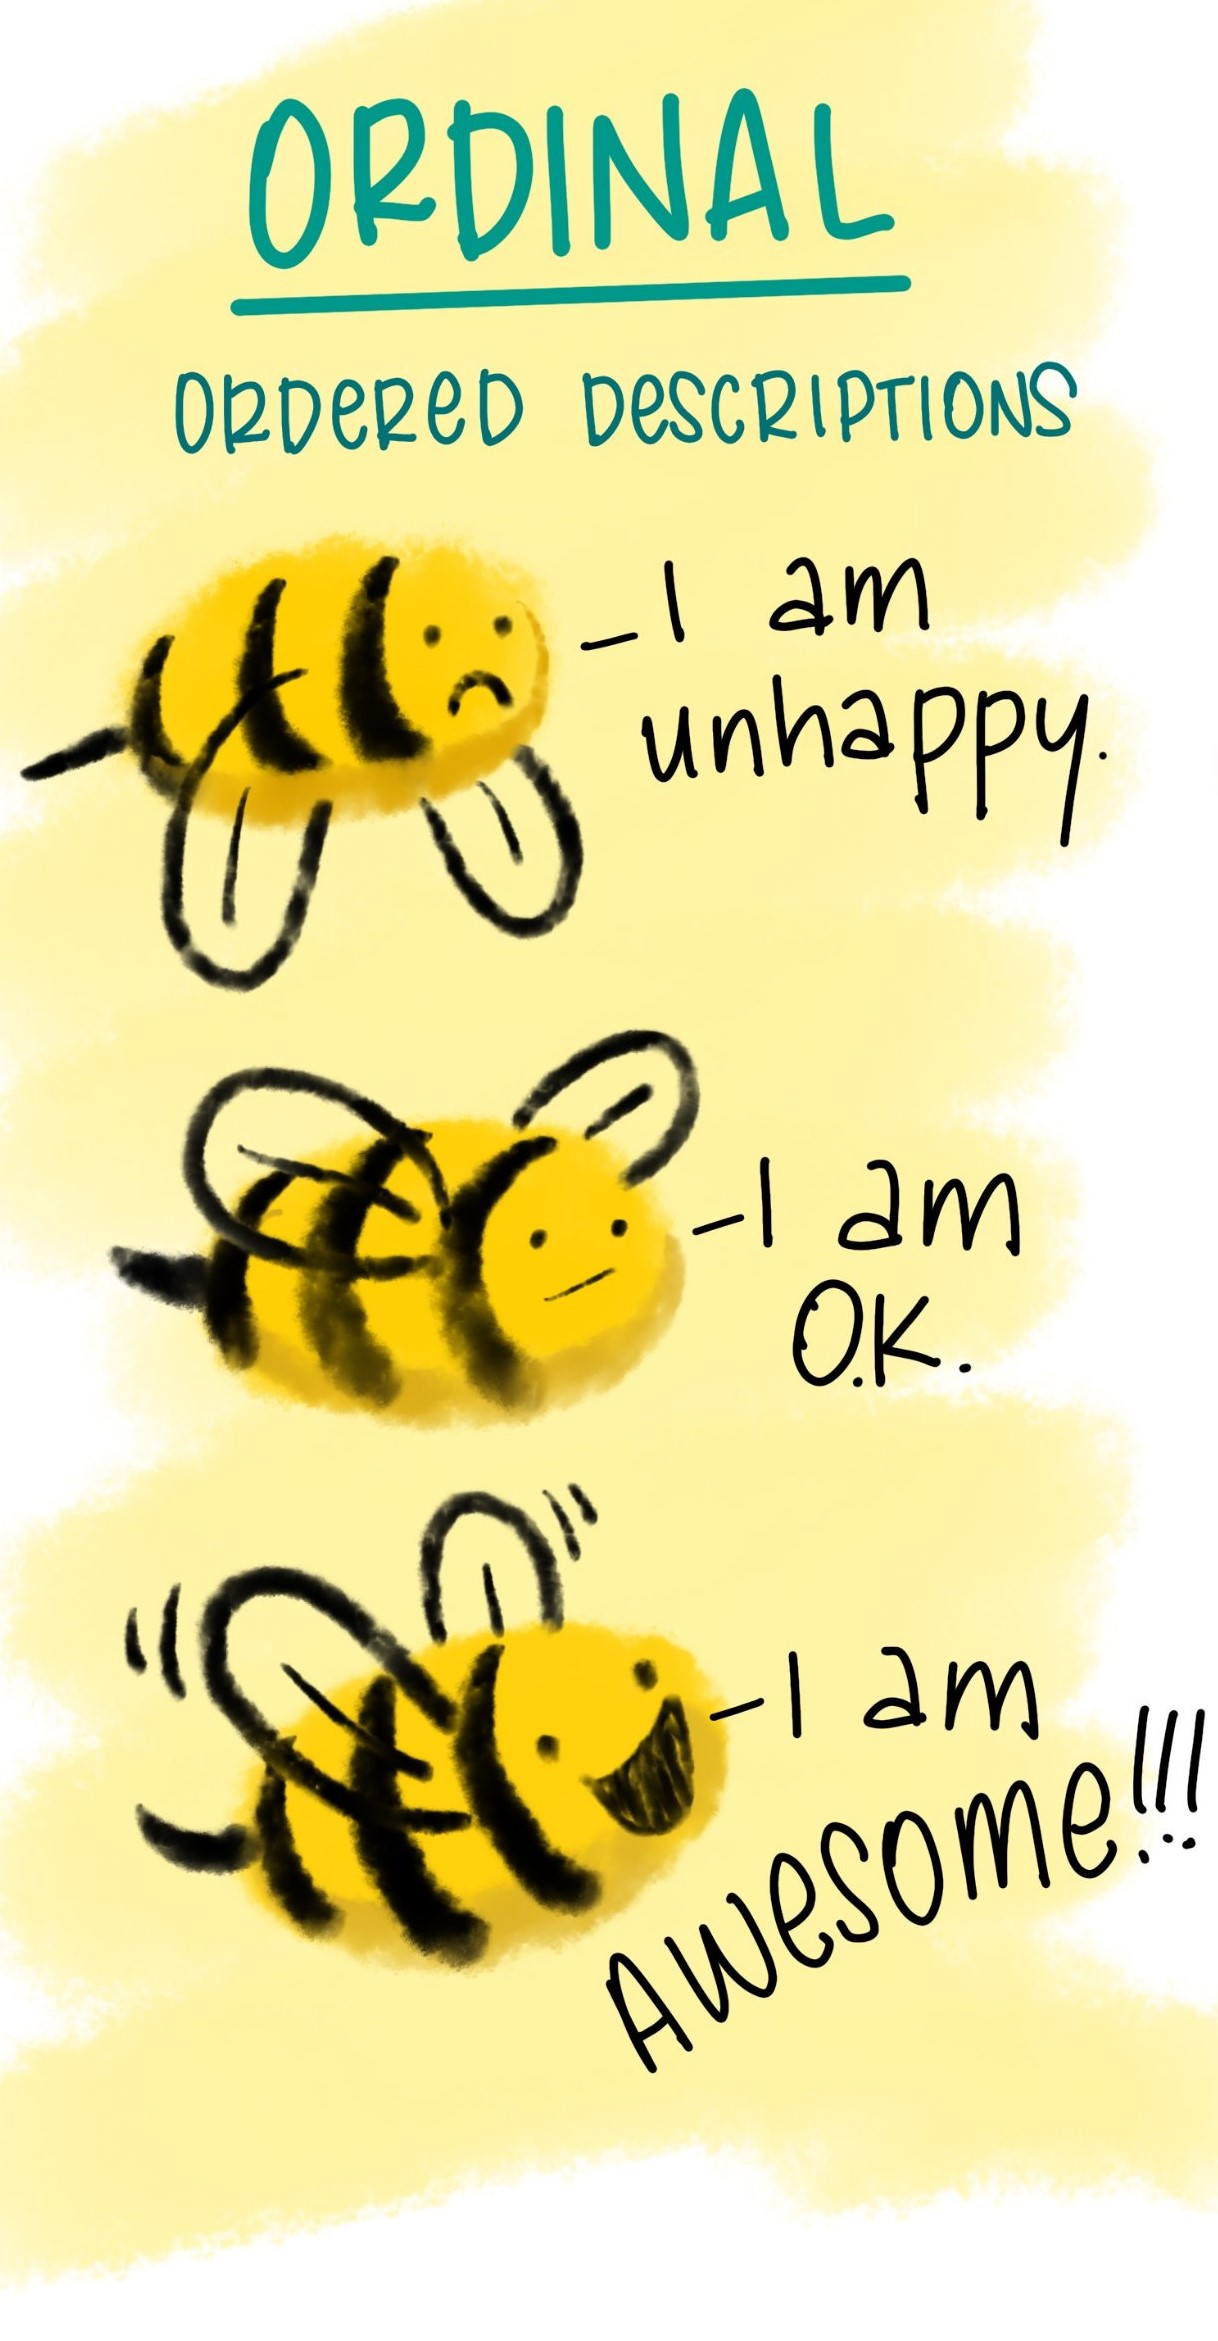
\includegraphics{../images/ord_copy.jpg}
\end{center}

\end{frame}

\begin{frame}

\begin{itemize}[<+->]
\tightlist
\item
  Modified Hachinksi

  \begin{itemize}[<+->]
  \tightlist
  \item
    0, 1, 2, 3 (in these data)
  \end{itemize}
\item
  Specific form of fuzzy coding: ``bipolar''
\end{itemize}

\end{frame}

\begin{frame}

\includegraphics{CA_MCA_Slides_files/figure-beamer/fake_hachinksi-1.pdf}

\end{frame}

\begin{frame}

\includegraphics{CA_MCA_Slides_files/figure-beamer/crisp_fuzzy_friends-1.pdf}

\end{frame}

\begin{frame}

\includegraphics{CA_MCA_Slides_files/figure-beamer/unnamed-chunk-14-1.pdf}

\end{frame}

\begin{frame}{Our second fuzzy friend}
\protect\hypertarget{our-second-fuzzy-friend}{}

\begin{center}
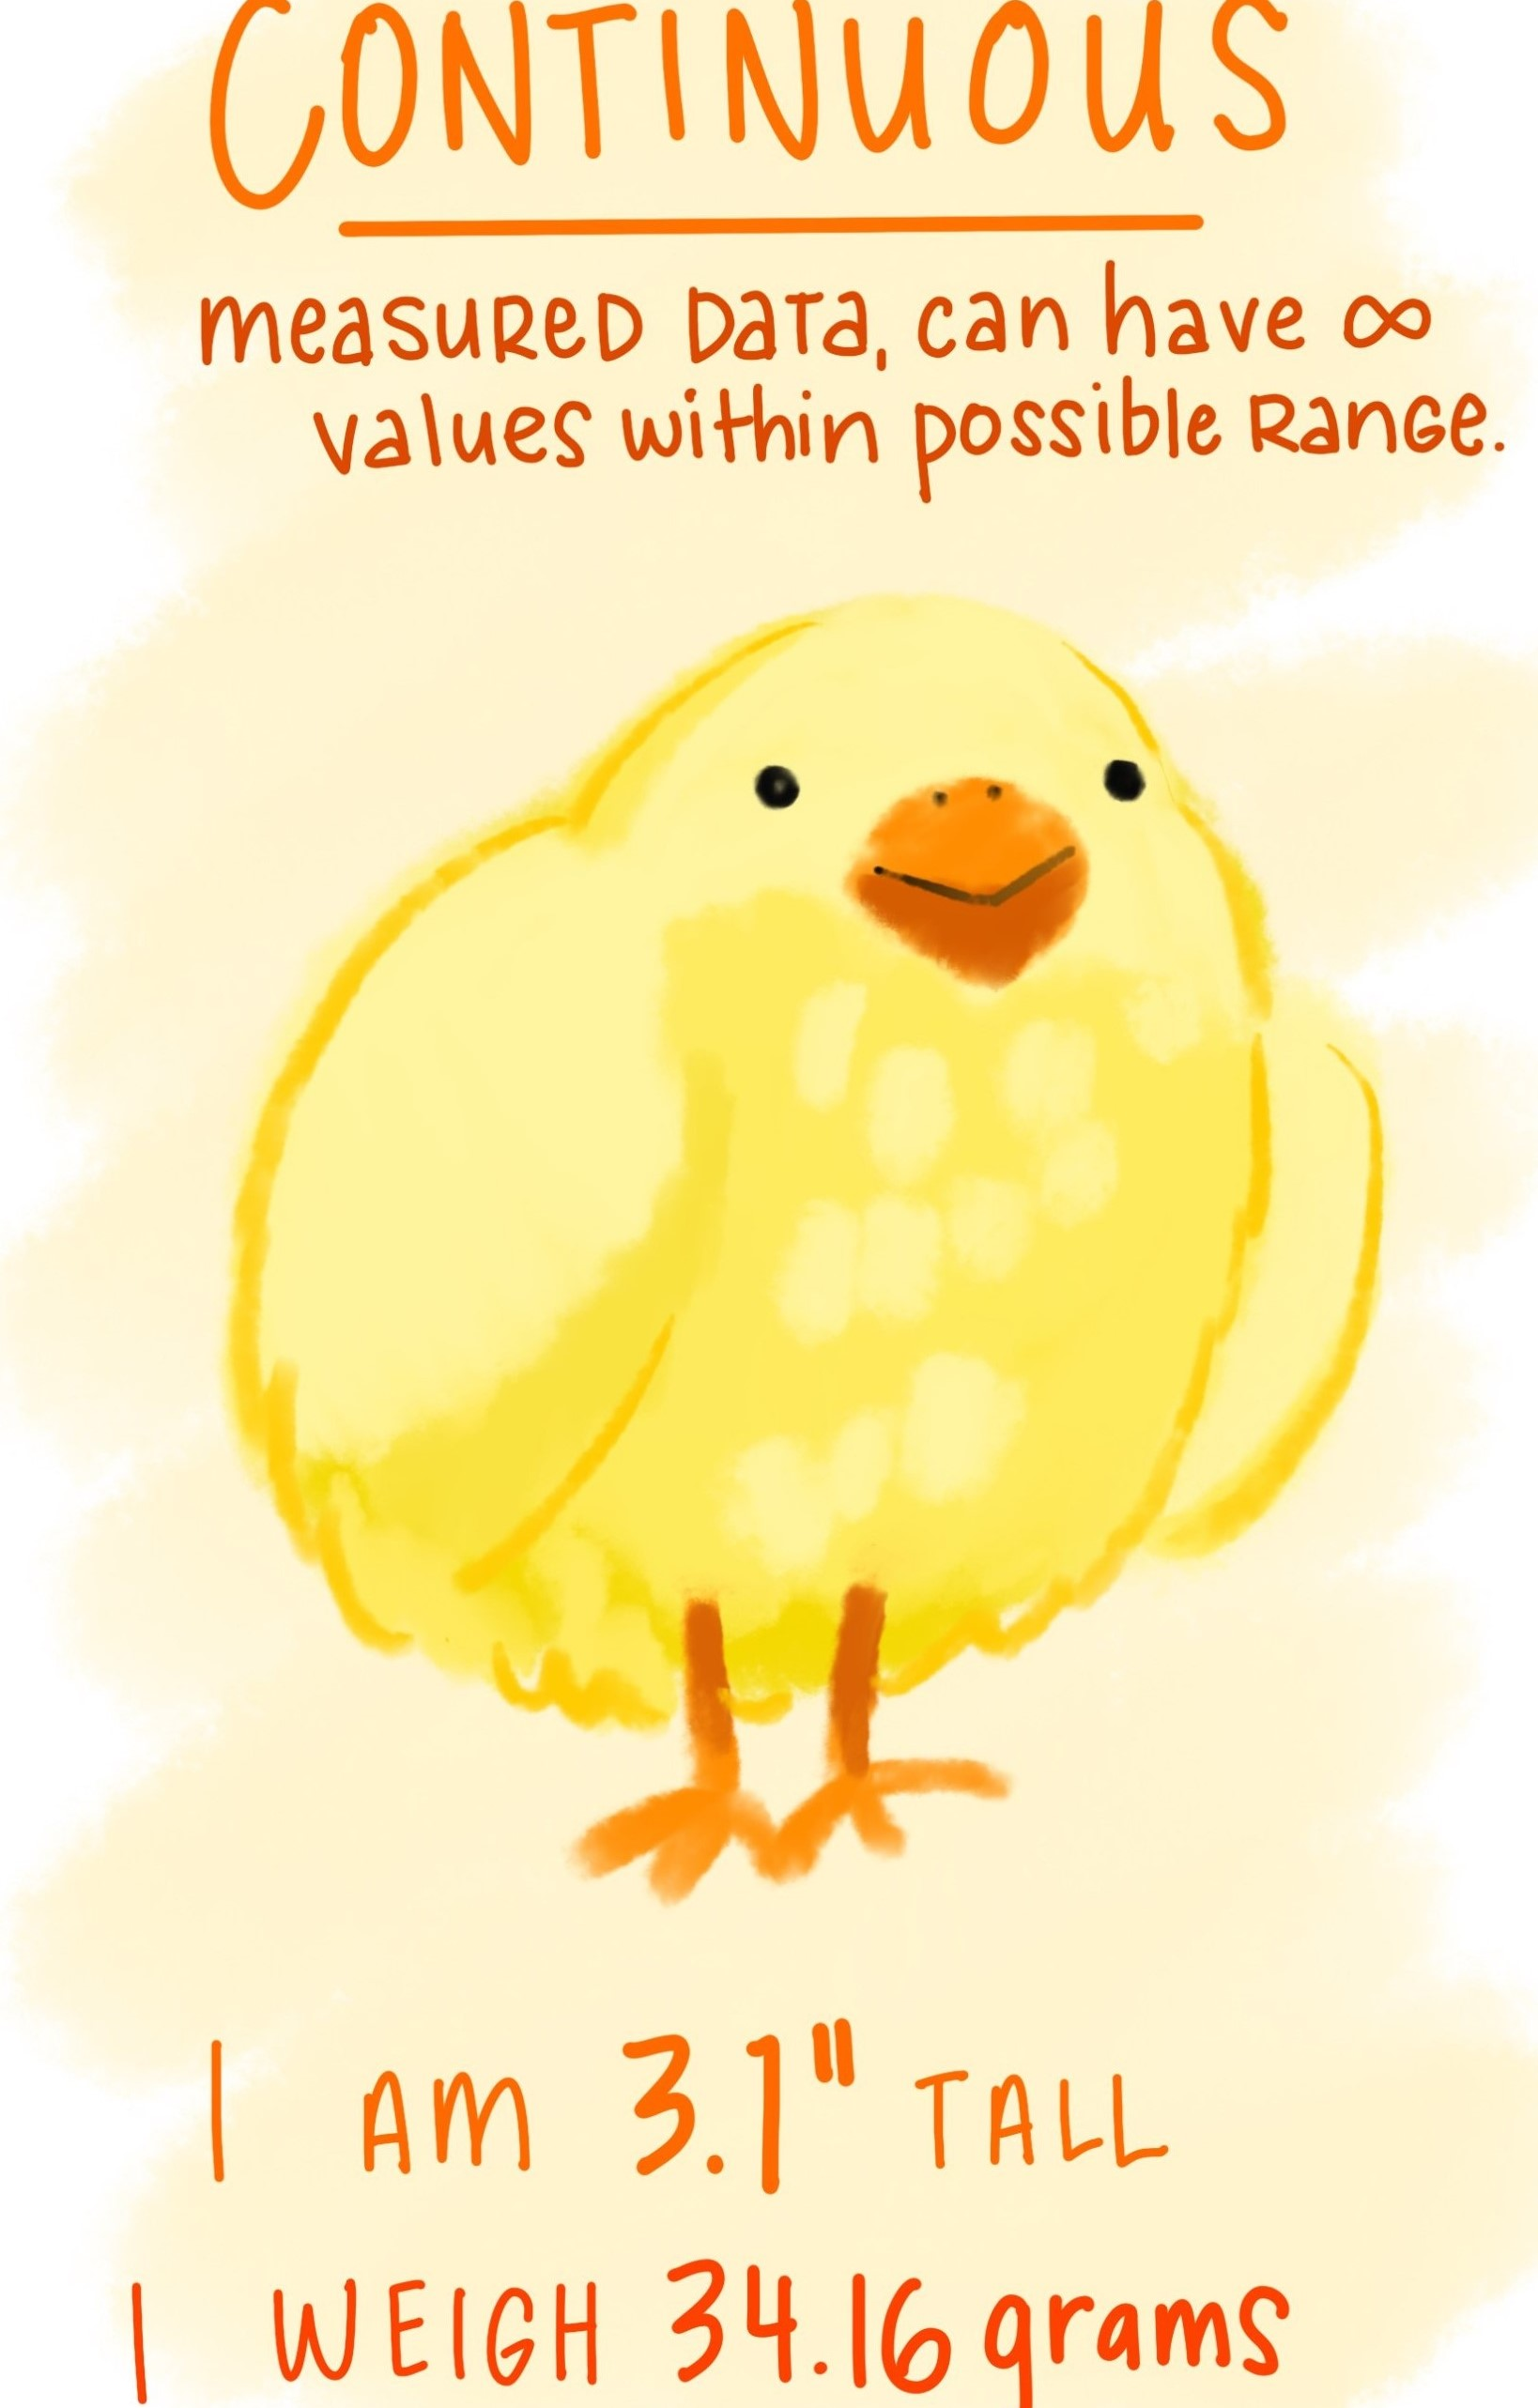
\includegraphics{../images/cont_copy.jpg}
\end{center}

\end{frame}

\begin{frame}

\begin{itemize}[<+->]
\tightlist
\item
  Age: 55.00 - 89.60

  \begin{itemize}[<+->]
  \tightlist
  \item
    But we need to scale it (Z-score)
  \end{itemize}
\item
  We use two columns again:

  \begin{itemize}[<+->]
  \tightlist
  \item
    \(\frac{(1 - x)}{2}\) \& \(\frac{(1 + x)}{2}\)
  \end{itemize}
\end{itemize}

\end{frame}

\begin{frame}

\includegraphics{CA_MCA_Slides_files/figure-beamer/fake_age-1.pdf}

\end{frame}

\begin{frame}

\includegraphics{CA_MCA_Slides_files/figure-beamer/crisp_fuzzy_x2_friends-1.pdf}

\end{frame}

\begin{frame}

\includegraphics{CA_MCA_Slides_files/figure-beamer/mca_mixed_2-1.pdf}

\end{frame}

\begin{frame}{How is this magic possible?!}
\protect\hypertarget{how-is-this-magic-possible}{}

\end{frame}

\begin{frame}

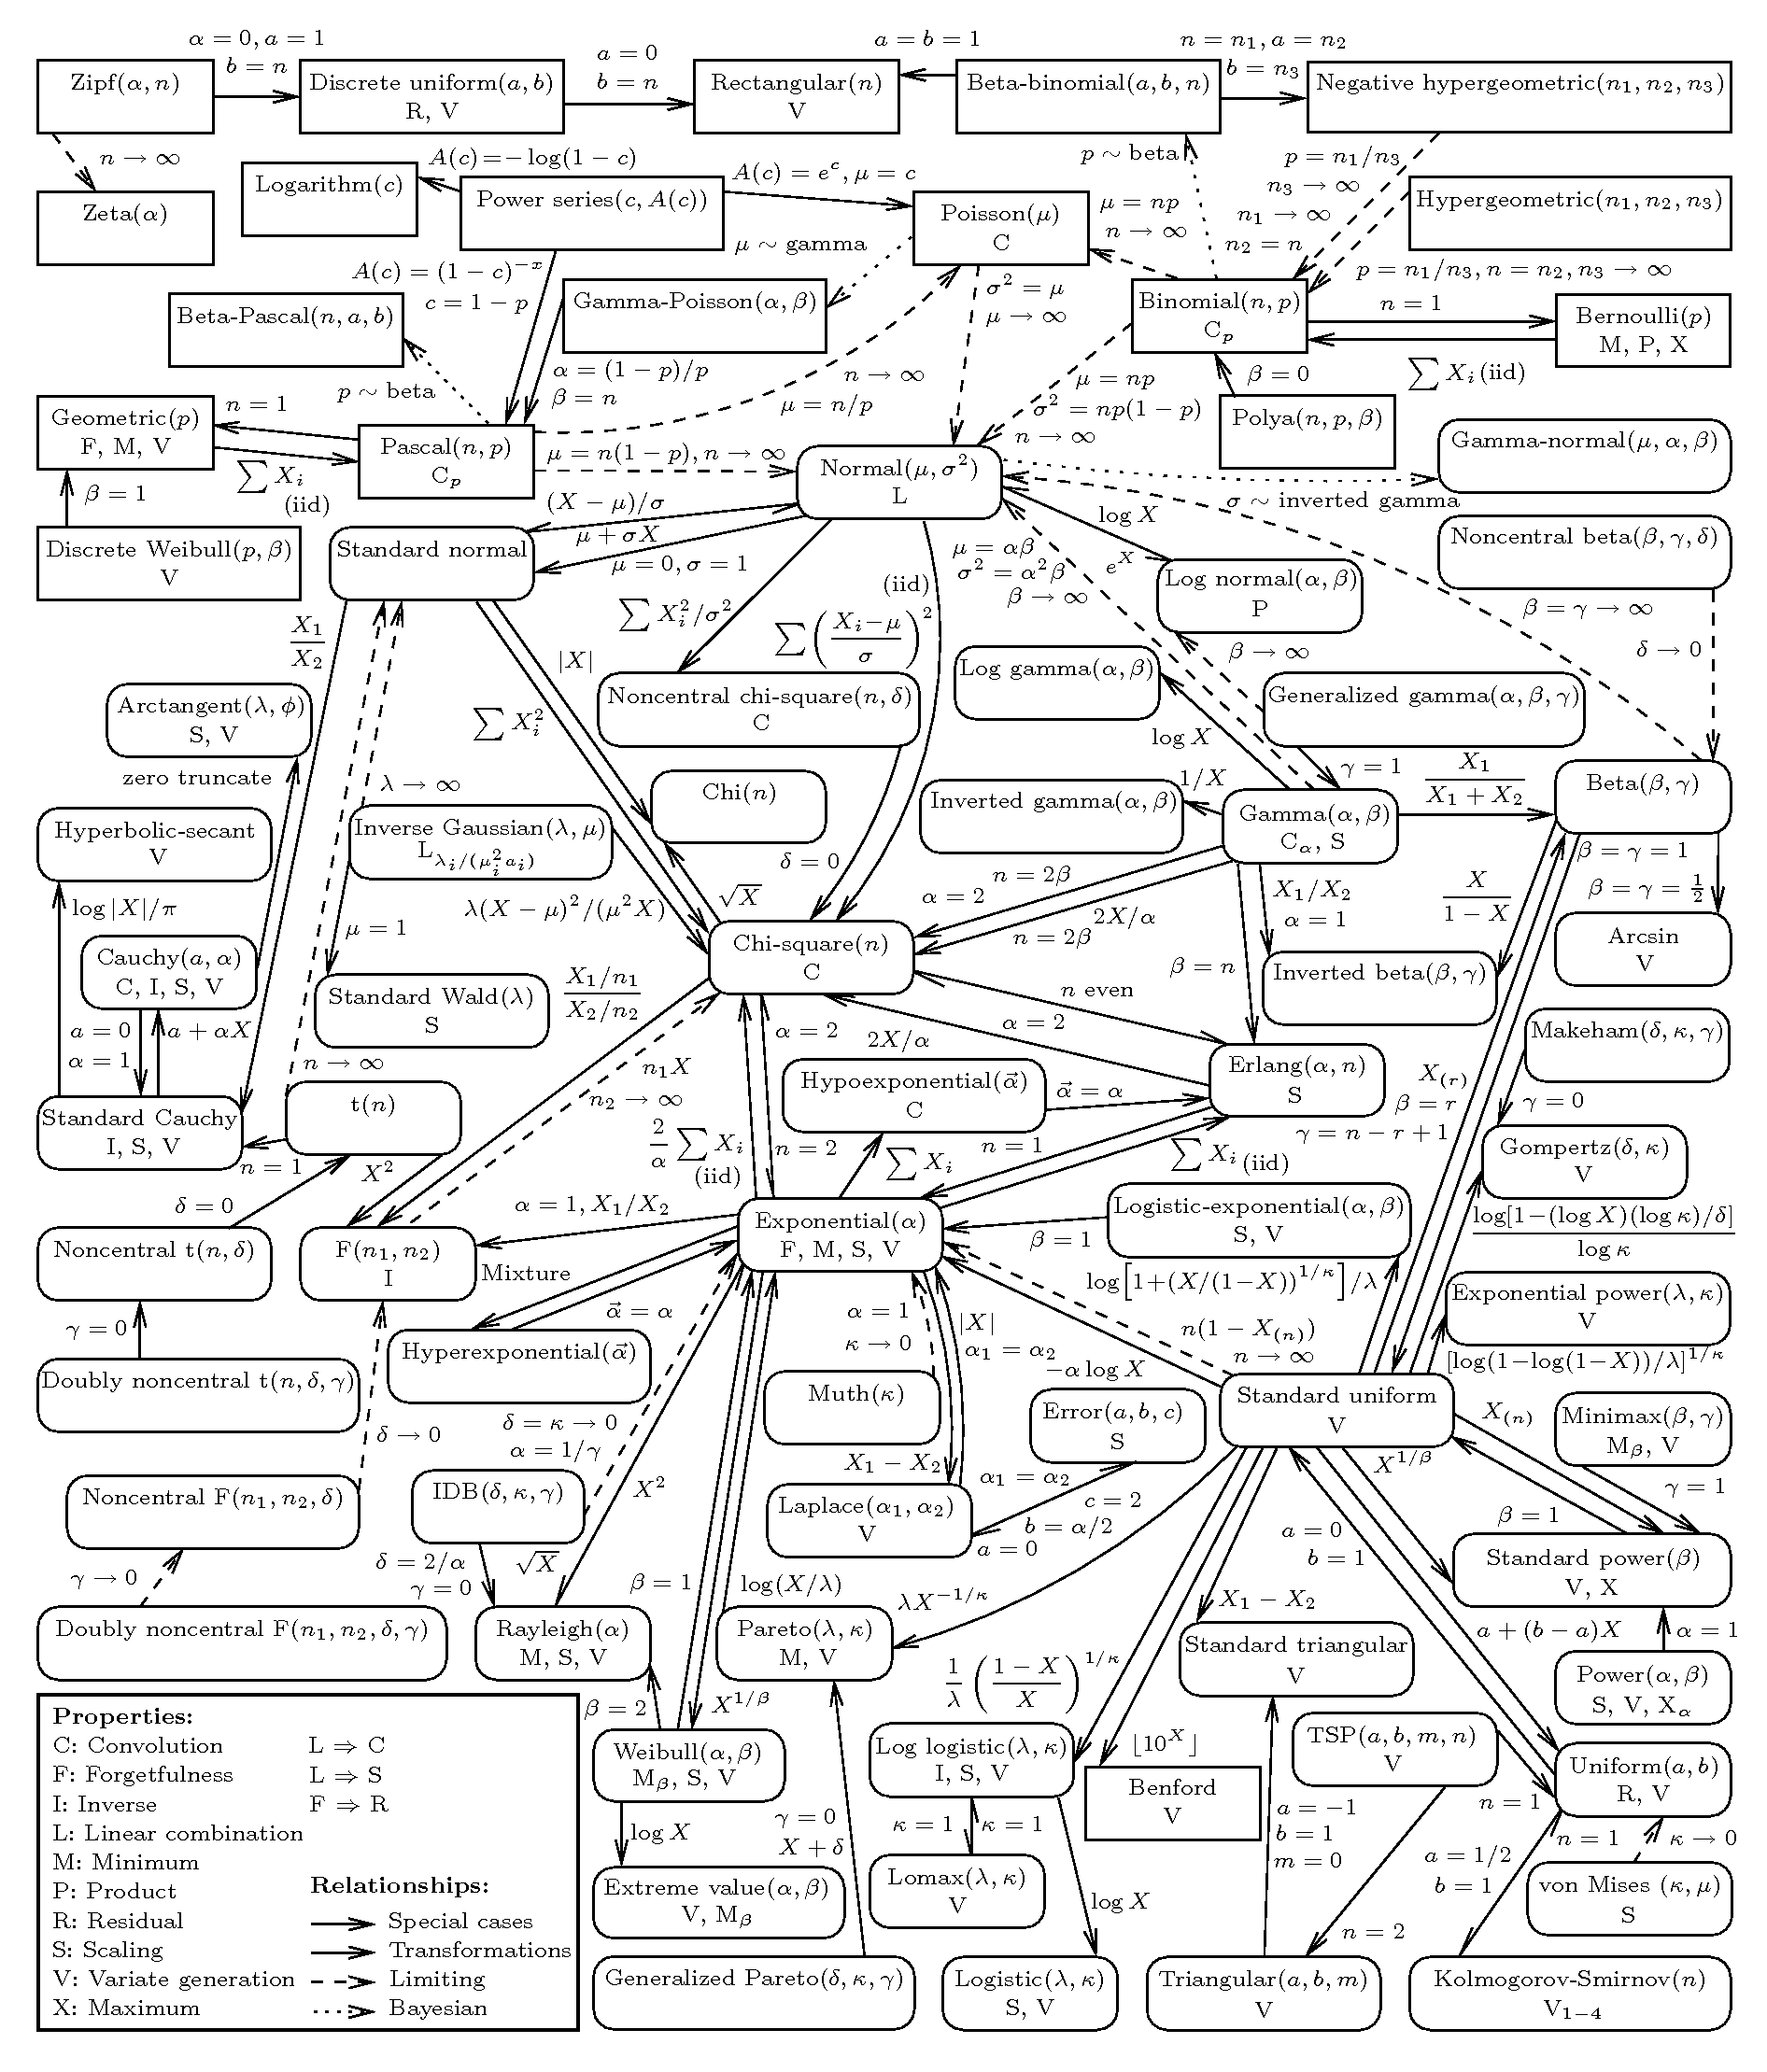
\includegraphics[width=\textwidth,height=0.75\textheight]{../images/distributions.png}

\href{http://www.math.wm.edu/~leemis/chart/UDR/UDR.html}{See here}

\end{frame}

\begin{frame}

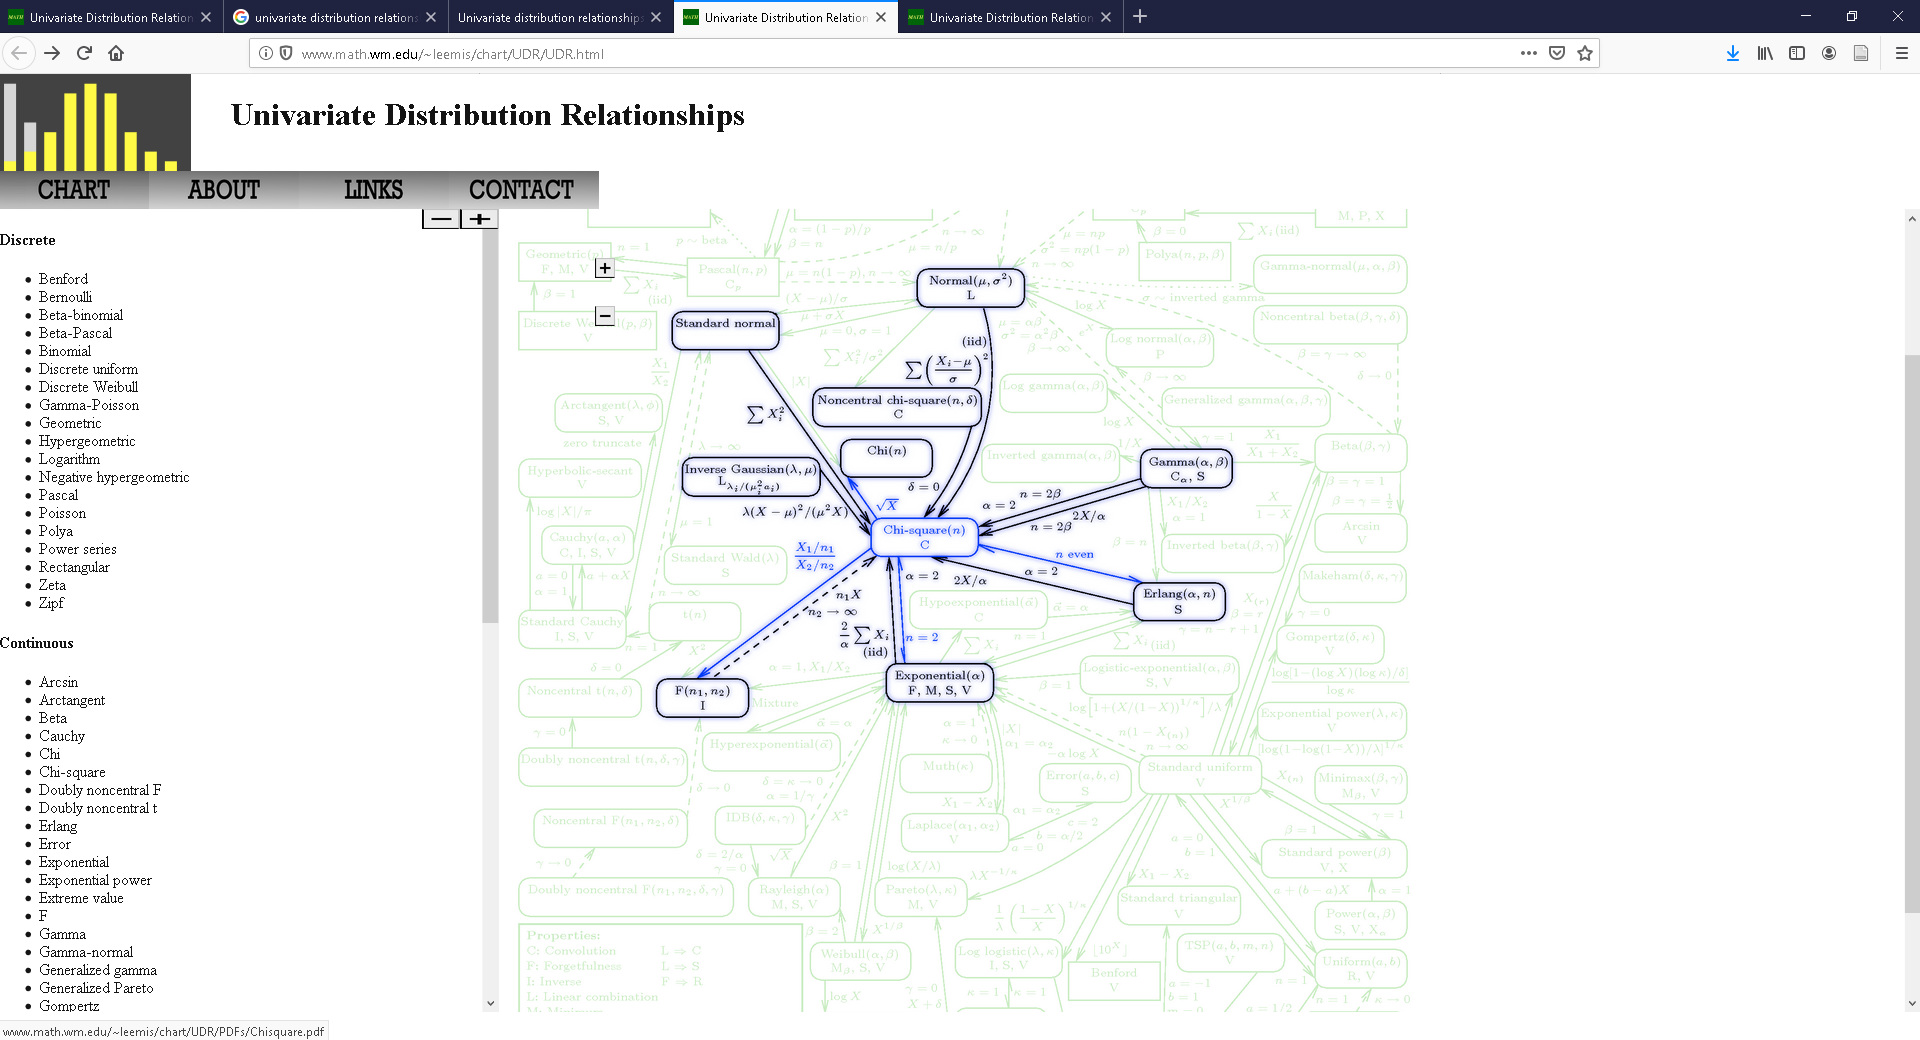
\includegraphics{../images/Chi2.PNG}

\href{http://www.math.wm.edu/~leemis/chart/UDR/UDR.html}{See here}

\end{frame}

\begin{frame}{Conclusions}
\protect\hypertarget{conclusions}{}

\begin{itemize}[<+->]
\tightlist
\item
  There's so much I'm not telling you

  \begin{itemize}[<+->]
  \tightlist
  \item
    I wish I could!
  \end{itemize}
\item
  But that's kind of the point

  \begin{itemize}[<+->]
  \tightlist
  \item
    CA is a \emph{massive} world
  \item
    Solves many problems we typically ignore
  \item
    And the \emph{G}SVD needs to be your other new best friend
  \end{itemize}
\item
  Learn to recognize data types

  \begin{itemize}[<+->]
  \tightlist
  \item
    Learn what to do with them
  \item
    But
  \end{itemize}
\end{itemize}

\end{frame}

\begin{frame}{Conclusions}
\protect\hypertarget{conclusions-1}{}

\begin{itemize}[<+->]
\tightlist
\item
  Ordinal---and ordinal like---are very difficult
\item
  Practical advice

  \begin{itemize}[<+->]
  \tightlist
  \item
    Small number of levels? Treat them as categorical
  \item
    HUGE number of levels? Inspect thoroughly
  \item
    In between? Probably ordinal
  \end{itemize}
\item
  Are they \emph{really} ordinal?

  \begin{itemize}[<+->]
  \tightlist
  \item
    Ranked, ordered? No inherent value?
  \item
    Or are these counts, discrete, imprecise continuous?
  \end{itemize}
\item
  What about:

  \begin{itemize}[<+->]
  \tightlist
  \item
    0, 1, 2, 3, 4?
  \item
    Never, Rarely, Sometimes, Frequently, Always?
  \item
    Use a mixture
  \end{itemize}
\end{itemize}

\end{frame}

\begin{frame}

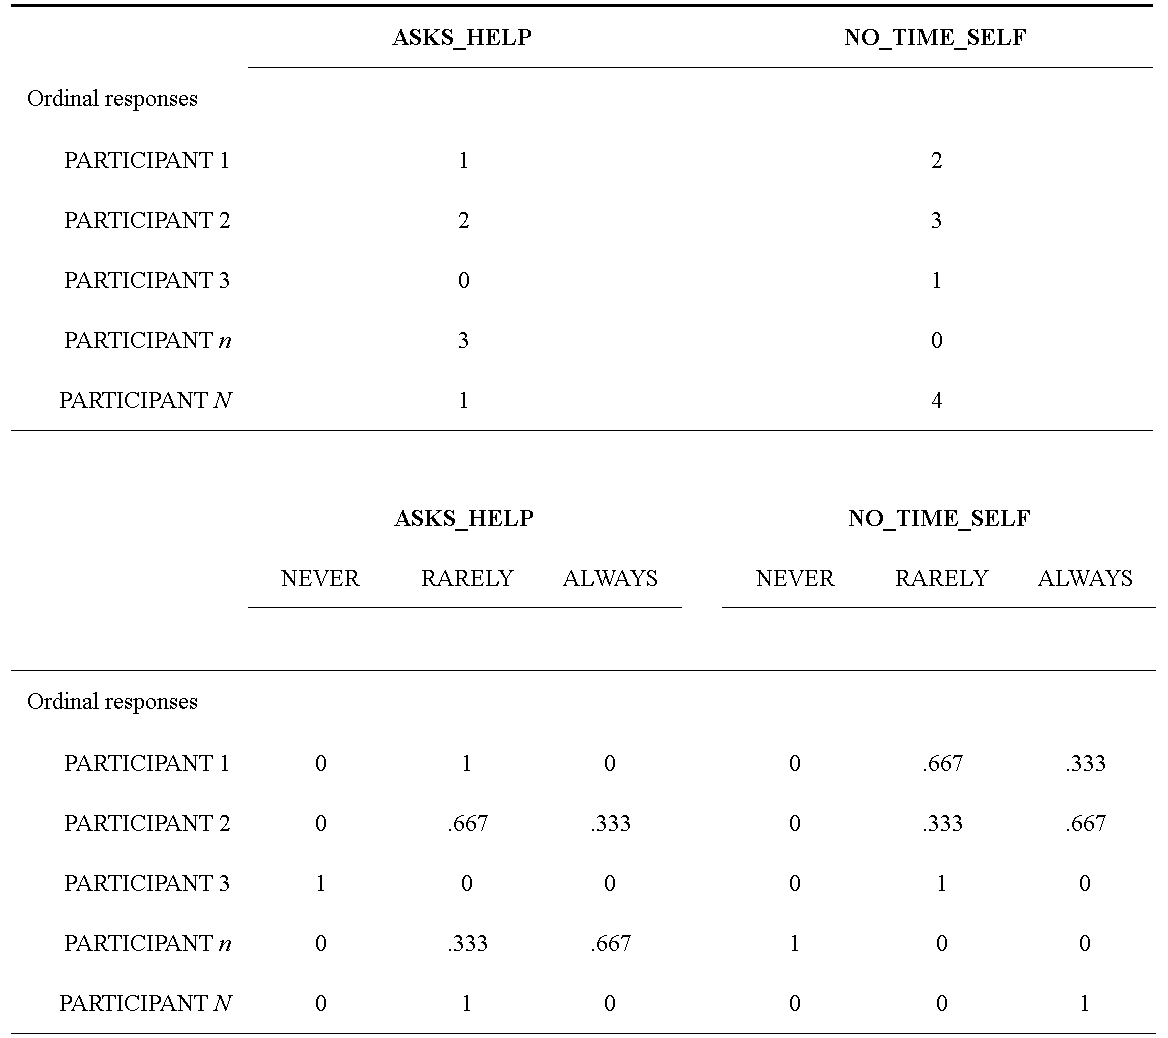
\includegraphics{../images/Fuzzy_Crisp_Mix.PNG}

\end{frame}

\hypertarget{some-many-bonuses}{%
\section{Some many bonuses!}\label{some-many-bonuses}}

\hypertarget{some-cool-stuff}{%
\subsection{Some cool stuff}\label{some-cool-stuff}}

\begin{frame}{A workshop}
\protect\hypertarget{a-workshop}{}

\begin{itemize}[<+->]
\tightlist
\item
  \url{https://github.com/derekbeaton/Workshops/tree/master/RTC/PCA_MCA_Resampling}

  \begin{itemize}[<+->]
  \tightlist
  \item
    Extraordinary detail on all of this
  \end{itemize}
\end{itemize}

\end{frame}

\begin{frame}{The Mueller report}
\protect\hypertarget{the-mueller-report}{}

\end{frame}

\begin{frame}

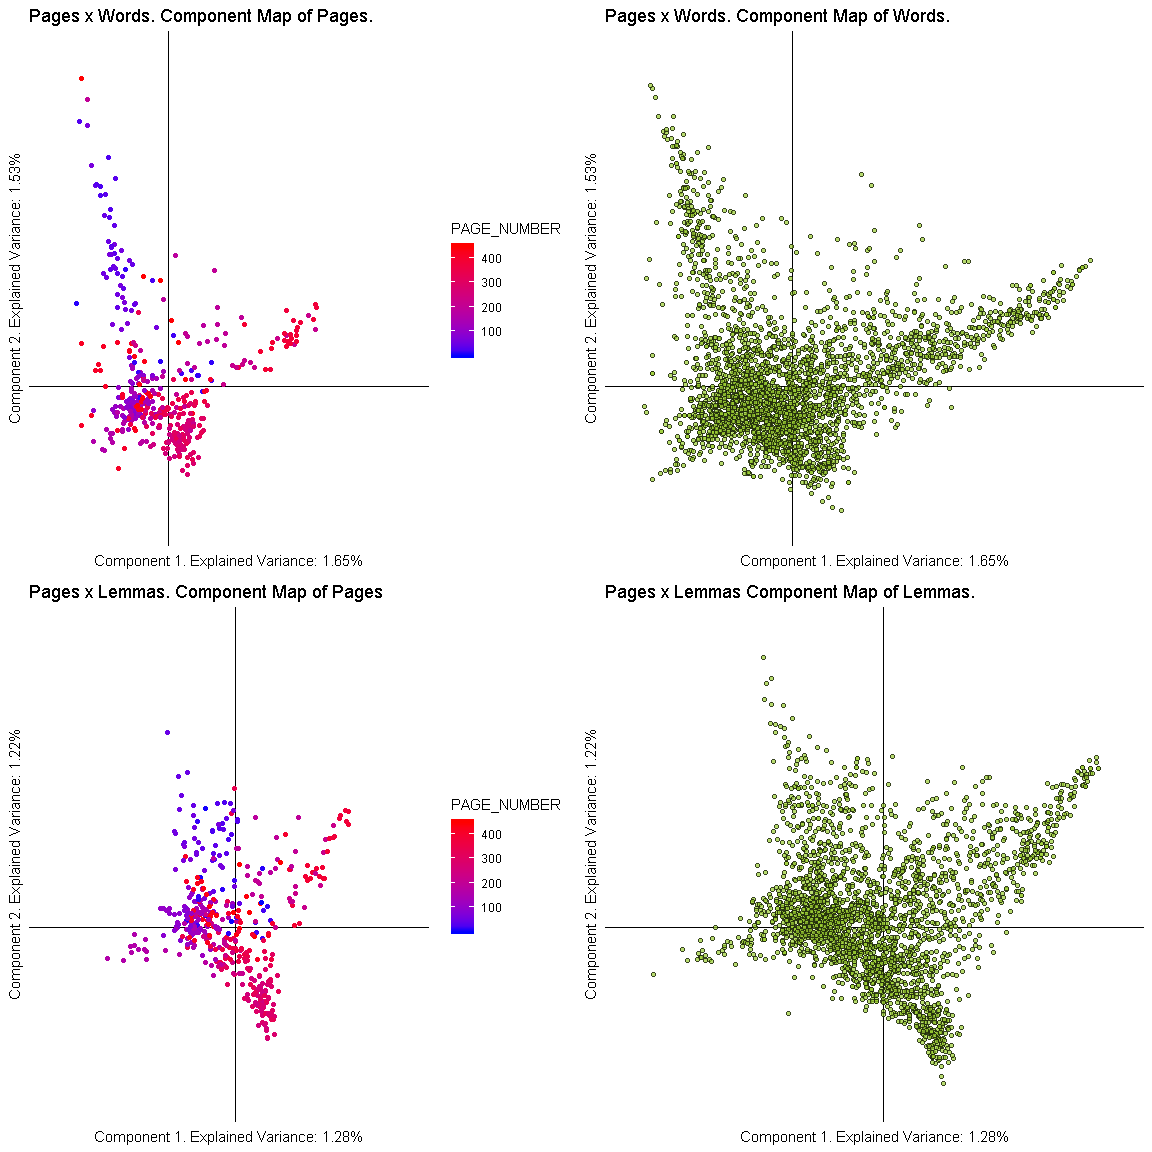
\includegraphics{../images/vis_components-1.png}

\href{https://github.com/derekbeaton/muellerreport_ca}{See here}

\end{frame}

\begin{frame}{The Marvel Cinematic Universe}
\protect\hypertarget{the-marvel-cinematic-universe}{}

\begin{itemize}[<+->]
\tightlist
\item
  Actually super cool
\item
  CA naturally handles networks
\item
  \url{https://github.com/derekbeaton/Marvel-Cinematic-Universe_Network/}
\end{itemize}

\end{frame}

\begin{frame}

\includegraphics{../images/2a_CA_12__NetworkConfig.png}

\end{frame}

\begin{frame}

\includegraphics{../images/3b_CA_78__NoGS_Min2_Network.png}

\end{frame}

\hypertarget{many-mixed-details}{%
\subsection{Many mixed details}\label{many-mixed-details}}

\begin{frame}{GMCD \& ours}
\protect\hypertarget{gmcd-ours}{}

\begin{itemize}[<+->]
\tightlist
\item
  Generalized minimum covariance determinant
\item
  ours (another R package)

  \begin{itemize}[<+->]
  \tightlist
  \item
    New package for outliers
  \item
    Has some important bells-and-whistles
  \item
    \url{https://github.com/derekbeaton/ours}
  \end{itemize}
\end{itemize}

\end{frame}

\begin{frame}{GPLS}
\protect\hypertarget{gpls}{}

\begin{itemize}[<+->]
\tightlist
\item
  First: a PLS for mixed data types

  \begin{itemize}[<+->]
  \tightlist
  \item
    Including those not discussed here
  \end{itemize}
\item
  Second: unify the ``two-table'' techniques

  \begin{itemize}[<+->]
  \tightlist
  \item
    PLS, CCA, RRR/RDA
  \end{itemize}
\item
  Package \& preprint

  \begin{itemize}[<+->]
  \tightlist
  \item
    \url{https://github.com/derekbeaton/gpls}
  \item
    Github issues where I routinely call myself a ``dummy''
  \end{itemize}
\end{itemize}

\end{frame}

\hypertarget{software}{%
\subsection{Software}\label{software}}

\begin{frame}{ExPosition}
\protect\hypertarget{exposition}{}

\begin{itemize}[<+->]
\tightlist
\item
  ExPosition

  \begin{itemize}[<+->]
  \tightlist
  \item
    Family of packages
  \item
    Includes resampling
  \item
    Lots of PCA \& CA techniques
  \end{itemize}
\end{itemize}

\end{frame}

\begin{frame}{Some alternatives}
\protect\hypertarget{some-alternatives}{}

\begin{itemize}[<+->]
\tightlist
\item
  FactoMineR
\item
  ade4
\item
  ca
\item
  MASS
\item
  psych
\item
  factoextra (visualization)
\item
  So many others
\end{itemize}

\end{frame}

\hypertarget{some-references}{%
\section{(Some) References}\label{some-references}}

\begin{frame}{Expansions \& data details}
\protect\hypertarget{expansions-data-details}{}

\begin{itemize}[<+->]
\item
  Beaton, D., Saporta, G., Abdi, H., \& Alzheimer's Disease Neuroimaging
  Initiative. (2019). A generalization of partial least squares
  regression and correspondence analysis for categorical and mixed data:
  An application with the ADNI data. bioRxiv, 598888.
\item
  Beaton, D., Sunderland, K. M., Levine, B., Mandzia, J., Masellis, M.,
  Swartz, R. H., \ldots{} \& Strother, S. C. (2019). Generalization of
  the minimum covariance determinant algorithm for categorical and mixed
  data types. bioRxiv, 333005.
\end{itemize}

\end{frame}

\begin{frame}{And these}
\protect\hypertarget{and-these}{}

\begin{itemize}[<+->]
\item
  Beaton, D., Fatt, C. R. C., \& Abdi, H. (2014). An ExPosition of
  multivariate analysis with the singular value decomposition in R.
  Computational Statistics \& Data Analysis, 72, 176-189.
\item
  Beaton, D., Dunlop, J., \& Abdi, H. (2016). Partial least squares
  correspondence analysis: A framework to simultaneously analyze
  behavioral and genetic data. Psychological methods, 21(4), 621.
\end{itemize}

\end{frame}

\begin{frame}{Techniques}
\protect\hypertarget{techniques}{}

\begin{itemize}[<+->]
\item
  Greenacre, M. (2017). Correspondence analysis in practice. CRC press.
\item
  Greenacre, M. J. (1984). Theory and Applications of Correspondence
  Analysis. Retrieved from
  \url{http://books.google.com/books?id=LsPaAAAAMAAJ}
\end{itemize}

\end{frame}

\begin{frame}{Techniques}
\protect\hypertarget{techniques-1}{}

\begin{itemize}[<+->]
\item
  Greenacre, M. J. (2010). Correspondence analysis. Wiley
  Interdisciplinary Reviews: Computational Statistics, 2(5), 613--619.
  \url{https://doi.org/10.1002/wics.114}
\item
  Lebart, L., Morineau, A., \& Warwick, K. M. (1984). Multivariate
  descriptive statistical analysis: correspondence analysis and related
  techniques for large matrices. Wiley.
\item
  Nguyen, L. H., \& Holmes, S. (2019). Ten quick tips for effective
  dimensionality reduction. PLOS Computational Biology, 15(6), e1006907.
\end{itemize}

\end{frame}

\begin{frame}{Data}
\protect\hypertarget{data}{}

\begin{itemize}[<+->]
\item
  Escofier, B. (1978). Analyse factorielle et distances répondant au
  principe d'équivalence distributionnelle. Revue de Statistique
  Appliquée, 26(4), 29--37.
\item
  Escofier, B. (1979). Traitement simultané de variables qualitatives et
  quantitatives en analyse factorielle. Cahiers de l'Analyse Des
  Données, 4(2), 137--146.
\item
  Greenacre, M. (2014). Data Doubling and Fuzzy Coding. In J. Blasius \&
  M. Greenacre (Eds.), Visualization and Verbalization of Data
  (pp.~239--253). Philadelphia, PA, USA: CRC Press.
\end{itemize}

\end{frame}

\begin{frame}{History}
\protect\hypertarget{history-1}{}

\begin{itemize}[<+->]
\tightlist
\item
  Holmes S, Josse J. Discussion of ``50 Years of Data Science''. Journal
  of Computational and Graphical Statistics. 2017, V26(4) 768-769.
  \url{https://www.tandfonline.com/doi/full/10.1080/10618600.2017.1385471}
\end{itemize}

\end{frame}

\end{document}
